%\bookmarksetup{startatroot}
\part{Thesis and Achievements}
%\setcounter{chapter}{0}

~\vspace{1cm}
\begin{flushright}
{\it A Scout is never taken by surprise: \\
he knows exactly what to do when anything unexpected happens.} \\ 
Sir Robert Baden-Powell
\end{flushright}
\vspace{2cm}

The study of the state-of-the-art in software engineering has highlighted the lack of a software solution to address all requirements identified in the context of home automation for Ambient Assisted Living. According to this observation, the goal of this thesis is to fill this gap by providing such a tool.\\

This section presents the achievements of this thesis. While the first chapter gives information about some central themes that drove this work, chapter~\ref{ch:detailsStrata} details the contribution. Then chapter~\ref{ch:outcomes} brings some information about the implementation and places the contribution in a classification framework.

\chapter{Contribution}


\section{Global ideas}

All throughout the work on this thesis some recurrent ideas drove both the search for solutions and the development of the proof of concept.

\subsection{Being inspired by electronics}

Variability, interoperability and adaptation are qualifiers that appear regularly in electronics. Indeed, any integrated circuit has to be able to operate with any other. Signals exchanged between components may have to be adapted, in order for the signal to reach the shape required by the receiver. Various solutions using many different electronic components can be envisioned to fulfil a need. People in this domain had to find and deploy tools, such as data-sheets or simulators, to eliminate these constraints.\\
This thesis was strongly inspired by this domain to come to a solution. The link between electronics solutions and the contribution of this thesis is stressed all throughout this section.

\subsection{Making it possible}

Scientific discoveries and advances are often due to hazardous reactions, unpredicted situations, and even due to errors. The software engineering tools of today limit runtime failures by cutting down the design elements to a set in which the interactions are well known. This mode of protection makes it difficult to design new systems, by using existing components in an unexpected way. Research or engineering phases must not be limited by these concerns.\\
This discussion can be compared with debates about static or dynamic typing in programming languages~\cite{Tratt:2009,Tratt:2010}: where static typing brings safety, it looses the flexibility of dynamic type systems.\\
This thesis work paid a strong effort in making type checking and validations policies highly flexible and customizable. It allows researchers and engineers to loosen checking rules, or deactivate validations to eliminate typing problems, and concentrate on experimenting new behaviors.

\subsection{Keeping end-users in mind}
\label{subsec:keepUserInMind}
Products are too often released to be sold, without end-users tests. As a result, these products may be considered too expensive or useless. From beginning to end, the solutions offered by this thesis have been designed for targeted users. Tools and methods were adapted to reduce the gap between how people are intended to behave and the way they actually use the solution.\\
Two populations of users have been particularly considered. The first population is the community of engineers and technicians which requires some tools to ease their work. Secondly is the system user population, such as carers and elderly people, who just want to be able to interact with the system. In both cases, it calls for the tools and the system to be highly intuitive. Intuitiveness has been improved by presenting the system to elderly people and by using the tools to design solutions.


\section{Overview of the contribution}

The contribution of this thesis is threefold. (1) A new component model, (2) tools to handle models, and (3) a runtime environment. To go into detail, these elements are presented as interacting layers. Each of them targets a particular concern and their synergistic collaboration makes the solution.
The different layers are visible in figure~\ref{fig:allLayersBig}, which provides an overview of the contribution.\\

\begin{figure}[h!]
  \centering
  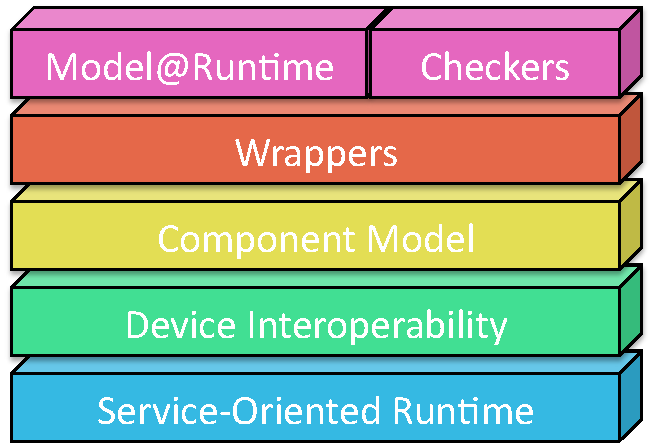
\includegraphics[width=.5\textwidth]{part2/pics/layers/AllBig.pdf}
  \caption{Overview of the EnTiMid layers}
  \label{fig:allLayersBig}
\end{figure}


{\bf Device Interoperability} addresses the mandatory need for {\it interoperability}. It is responsible for communication with real devices and their representatives in the {\it Component Model}.\\

The {\bf Component Model} involves structures and methods, to handle abstract representations of real devices. It provides a unified description of available ports, parameters, and any other useful information for the {\it Model@Runtime} layer to work in good conditions. It enables the creation of tools to cope with variability, interoperability and safety concerns.\\

The {\bf Model@Runtime \& Checkers} layer concerns the necessary tools to ease the management of the system. The implementation specificities of components are invisible at this level, thanks to the {\it Component Model} layer. Simulations and checks can be safely performed at this level of abstraction, with no consequences on the running application. Model@Runtime enables the management of the system while running, and helps in dealing with variability management. Checkers offers tools for validation and improvements for the safety of the solution.\\

The {\bf Wrappers} layer takes responsibility for publishing the devices present in the system, on application level networks. This ability opens our solution to existing and future, protocols and evolutions. Often too heavy to be embedded, this layer offers the devices, for free, an access through application level protocols.\\

The {\bf Service Oriented Runtime} completes the contribution, by offering an execution environment for the new component model. It brings "life to the {\it Model@Runtime}" by providing the support for dynamic {\it adaptations} and {\it evolutions} while running.\\

Each level participates in meeting the requirements identified in chapter~\ref{ch:requirements}. Table~\ref{table:layer_req} shows what concern is addressed by each layer. Separately, each layer does not satisfy all needs, but their collaboration does.\\

\begin{table}[h!]
\begin{tabular}{m{.20\textwidth}| >{\centering\arraybackslash}m{.12\textwidth}| >{\centering\arraybackslash}m{.07\textwidth}| >{\centering\arraybackslash}m{.09\textwidth}| >{\centering\arraybackslash}m{.08\textwidth}| >{\centering}m{.11\textwidth}| >{\centering\arraybackslash}m{.12\textwidth}|}
 {\it Takes part in}& {\tiny Interoperability} & {\tiny Openness} & {\tiny Adaptation} & {\tiny Evolution} & {\tiny Variability Management} & {\tiny Safety \& Security}\\
 \hline\hline
 {\small Model@Runtime} & & & + & + & + & + \\
  \hline
 {\small Wrappers} & & + &  & + &  & \\
  \hline
 {\small Component Model} & + & & + & + & & \\
  \hline
 {\small Device Interop.} & + & & & & & \\
  \hline
 {\small Service-Oriented Runtime} & & & + & + & &\\
 \hline
\end{tabular}
 \caption{Mapping layers to requirements}
 \label{table:layer_req}
\end{table}

%\begin{wrapfigure}{r}{40mm}
%  \vspace{-4mm}
%  
\includegraphics[width=40mm]{part2/pics/entimidLogo.png}
%  %\vspace{-5cm}
%\end{wrapfigure}

\par This contribution has been implemented. The runtime, called \enti{}, has been developed on top of an OSGi platform. By the way, \enti{} is a compound word from the Breton "En Ti", which means "In house", and "Mid", for Middleware. It is thus the middleware in the house. The component model has been developed using classical modeling techniques. Tools have been created to enable all functionalities.\\
Chapter~\ref{ch:detailsStrata} details each layer of this contribution.


\chapter{Details on strata}
\label{ch:detailsStrata}


Like a geologist, this chapter dissects the contribution layer by layer. For each stratum composing the proposal, a section gives details on the roles taken on by the layer, its achievements, and its interactions with other strata.\\

The first section starts with the description of the Device Interoperability layer, which takes an essential role in the contribution since it enables heterogeneous connections. Section~\ref{sec:componentModel} then details the different concepts present in the component model, their interactions, and describes how the synchronization between component implementations and models is guaranteed. Section~\ref{sec:martAndReasoning} explains how the Model@Runtime and Reasoning layer takes advantage of the component model to offer a great flexibility and multiple points for checking the conformance. The runtime environment chose is briefly presented is section~\ref{sec:soaruntime}, while section~\ref{sec:wrappers} introduces the Wrappers layer.

\section{Device Interoperability}

\begin{wrapfigure}{r}{60mm}
  \vspace{-5mm}
  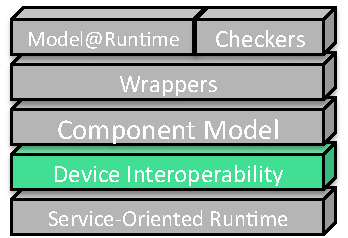
\includegraphics[width=60mm]{part2/pics/layers/DevicesInterop.pdf}
%  \caption{Interoperability Layer}
%  \label{fig:interopLayer}
  \vspace{-5mm}
\end{wrapfigure}

The Device Interoperability layer is probably the most important layer of the approach, since it answers the first requirement. Variability management, adaptations, or evolutions, would be compromised if only two devices were not able to communicate. Interoperability of devices is a central concern. It offers a foundation on which other layers can be built. This section presents how this interoperability has been realized.\\

In the domain of home automation, communication protocols used by manufacturers and their devices are not compatible. This incompatibility makes any direct interaction of devices coming from different brands impossible. To overcome this barrier, some manufacturers have worked in a consortium to define a unique communication protocol for their respective products to be compatible. However, some of their products code Boolean values on a single bit, while others code it on a byte. Again, two products may not be operable with each other.\\
In~\cite{Bromberg:2009} Bromberg et al. propose to automatically generate gateways between protocols, in order to address this issue. But building protocol-to-protocol translators solves the problem only partially, because the number of translators exponentially explodes with the number of protocols. Nevertheless, this proposition seems very interesting for an automatic generation of translators, from specific protocols to a higher-level of abstraction model.

\subsection{Use of drivers}
\label{subsec:useOfDrivers}
To realize this abstraction, drivers have been developed. A driver makes the link between real world devices and their virtual representation in a software system. Thus, they take on two responsibilities. In one way, they convert from vendor-specific communication messages to actions on their virtual representative. They also translate in the other way, actions on virtual elements into vendor-specific messages. \\
Secondly, drivers provide the virtual structures for each product they are able to interact with. All implementations specific to a given manufacturer are thus contained in drivers, or separate libraries. This makes the core system completely independent from devices' implementation specificities.\\

This independence implies the creation of a common structure, for the system to be able to properly handle devices in a good abstraction level.

\subsection{Functional interfaces}

This common structure may take the form of a set of programming interfaces. Each interface could specify a set of methods for a specific functionality. Then, drivers just have to provide objects, decorated with some interfaces, selected according to the abilities of each device. This set of programming interfaces has been created. A survey of devices functions has allowed us to extract the minimum set of common methods for each function as presented in figure~\ref{fig:interfaces} for instance. Once the set is defined, a library containing all interfaces was compiled and included in the framework.\\
\begin{figure}[h!]
\centering
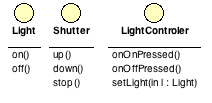
\includegraphics{part2/pics/FunctionalInterfaces.png}
\caption{Functional Interfaces}
\label{fig:interfaces}
\end{figure}
The first experiments were promising. Interoperability was almost solved, but several drawbacks were rapidly identified while using this approach in real use cases. The set of interfaces is only extensible by augmentation of the framework. The development of a device driver could have fail because the required function interface was not available in the library. Moreover, direct method calls are not appropriate if the system has to consider a dynamic environment, in which objects unpredictably appear and disappear. In this case, object-oriented development using synchronous method calls becomes quite hazardous. Finally, if for any reason a component implementing the {\it LightControler} interface has to be plugged into a shutter, the operation is not feasible without an ad-hoc adapter (illustrated in figure~\ref{fig:interfaces}). Interoperability was not solved.\\


\subsection{Event-based approach}

Real-life events can occur in any order, at any time, in any context. Moreover, devices are more and more mobile and can dynamically join or quit the system. In order to address this dynamicity, we made use of event-based mechanisms. \gls{mom} offers a simple, and efficient means of communications, using the publish/subscribe principle. Event consumers subscribe to a topic they are interested in, and event producers just have to publish on the right topic. Thus, producers do not care about the presence of consumers.\\
To be able to use this approach, physical devices have been considered from two perspectives. {\it Sensors} sense real life and human actions. Their role is to feed the system with events coming from real life. They are producers of events. Consuming these events, {\it Actuators} act on real life, using real-life equipment. They carry out orders such as switching on the lights, or opening or closing the shutters. 
Components are not limited to a unique role, and can both consume and produce events.\\

{\bf Actuators} propose two main methods. {\it getAvailableActions()} returns a list of actions that can be carried out on the device. If a light can answer [{\it on,off}], a shutter could answer [{\it up,down,stop}]. For each action, actuators wait for messages on a specific topic. For a sensor to ask for an action to be realized, it must know the corresponding topic. {\it getTopicFor(String action)} aims at providing the topic and the parameters that can be accepted for a given action in form of a {\it Message}.\\

{\bf Sensors} maintain a list of messages for each event they sense. An On/Off switch maintains two lists of messages: one for each action. The messages stored also embed the topic on which they have to be published, for the action to be carried out. When an action is sensed, each message stored for this action is sent on its topic.


\subsection{Example}

For instance, figure~\ref{fig:seqDiagConfMom} shows the configuration phase for the connection of a switch and a light. The \textit{Configurator} retrieves the message to be sent to switch on the light. This message is added to the list of the "on" sensed value of the switch. Later, when the "on" button is pressed, all messages stocked in the list are sent. When an actuator recognizes its "on action message", it forwards the order to the real light.\\

\begin{figure}
\centering
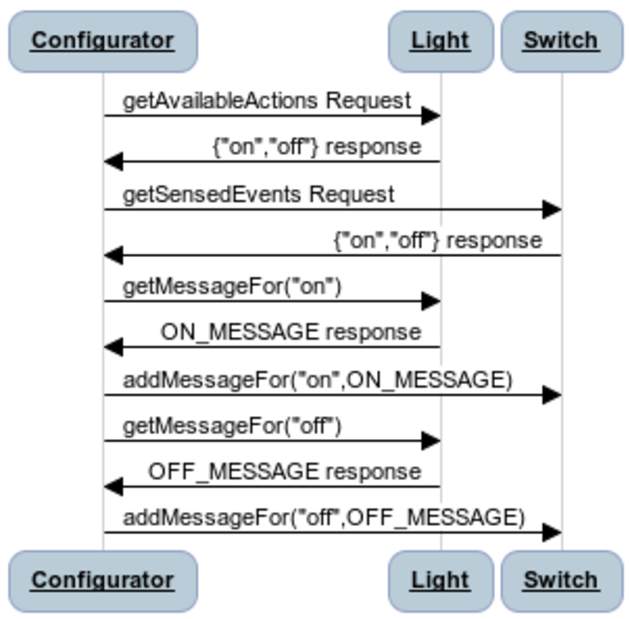
\includegraphics[width=.5\textwidth]{part2/pics/SequenceDiagram.pdf}
\caption{Configuration Phase}
\label{fig:seqDiagConfMom}
\end{figure}

This mechanism allowed us to eliminate asynchronous aspects. It also allowed any sensor to control any actuator, since they do not have to know each other to be able to work together. The action carried out and the value sensed do not have to necessarily be the same. Thanks to the mechanism of messages, it is possible to send the "on" message to the light when "down" is sensed by a shutter command.\\

\begin{figure}
\centering
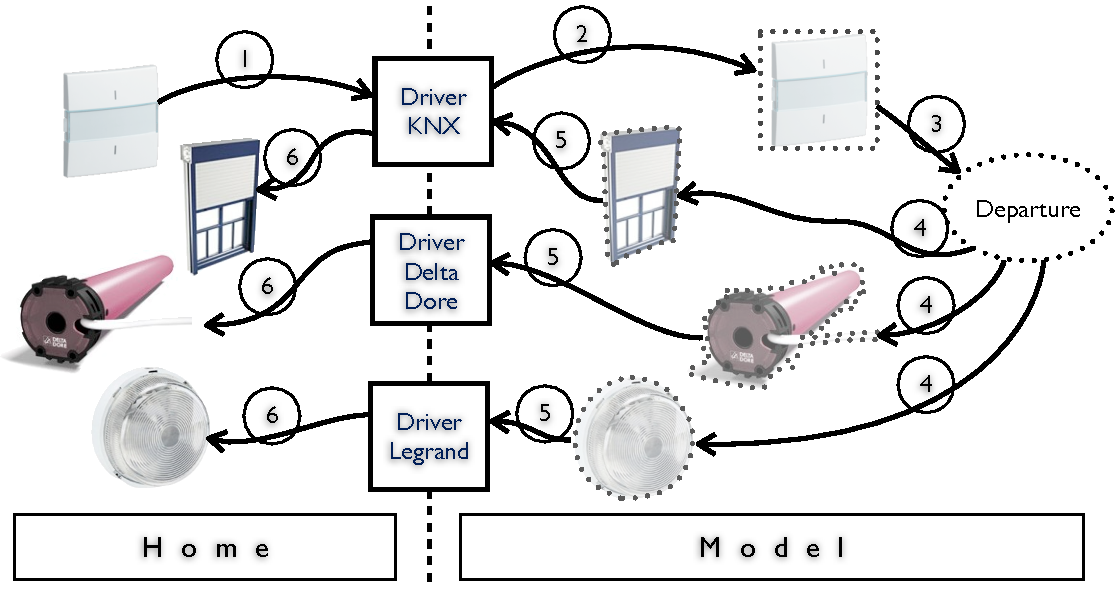
\includegraphics[width=.8\textwidth]{part2/pics/InteropExample}
\caption{Example of Interoperability}
\label{fig:interopExample}
\end{figure}


Let us consider a home with a switch to trigger a departure scenario, operable on the KNX network. This scenario switches off all lights and closes shutters. In the considered example, there are only two shutters and one light. The first shutter was motorized when the house was built and works on a KNX network. The second shutter was added afterwards and as the owners did not want to make holes in the walls, they chose a shutter engine communicating with the command by radio frequencies. Lastly, lights are controlled by Legrand equipment. All these elements are visible on the left of figure~\ref{fig:interopExample}.\\
The interoperation of all these elements is described in the case of a departure scenario activation. Numbers on the figure present the sequence of actions.\\
{\bf 1-} An inhabitant presses the button. This action is sensed, and generates a message on the KNX network.\\
{\bf 2-} This message is read by the driver and translated into a message for the EnTiMid system.\\
{\bf 3-} The driver then selects the virtual representation of the device responsible for the message and activates the sending of stored messages.\\
{\bf 4-} Its activation causes all connected elements to be activated in parallel.\\
{\bf 5-} On receiving the message, each model representative of a real product asks its driver to send an order to the real product.\\
{\bf 6-} The driver executes the query and sends the order.\\
In this example, various devices with various actions are connected together. A switch that senses a {\it departure} is connected to two {\it down} actions on two different components and one {\it off} port. Interactions between components are possible thanks to the exchange of messages.\\

\subsection{Threat to validity}
Interoperability was tested and validated with a restricted set of devices. Since the main goal of this thesis is not about making any device interoperable, the study was conducted with a set of representative technologies mixing different communications media, different appliances and multiple manufacturers, in order to prove the feasibility. 

\subsection{Summary}

The {\it Device Interoperability} layer enables products from any manufacturer to work with any other product, in any imaginable way, by just implementing a driver. The use of this method is however limited by the non-availability of action lists at design time. Each device provides information about the actions it supports, but a method has to be called. Since method calls cannot be done at design time, the only way to obtain available actions is to go and seek them in the implementation code.\\
The sequence diagram, presented in figure~\ref{fig:seqDiagConfMom}, describes a part of the work that a piece of program has to execute to set up the application's behavior. The sequence cannot be implemented definitively, since the application may have to be adapted and to evolve while running. The configuration has to be expressed another way, to be modifiable, and to ease the reading and understanding of the behavior.\\

Both of these issues require a tool. It has to be able to provide information about the devices at design time, and it has to support and help device assembly design. This tool, a new component model, is made available by the {\it Component Model} layer.

\newpage
\section{Component Model}
\label{sec:componentModel}
\begin{wrapfigure}{r}{60mm}
  \vspace{-8mm}
  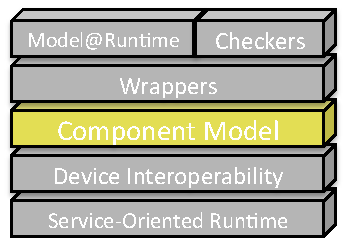
\includegraphics[width=60mm]{part2/pics/layers/ComponentModel.pdf}
%  \caption{Component Layer}
%  \label{fig:componentLayer}
  \vspace{-8mm}
\end{wrapfigure}

On top of the {\it Device Interoperability} layer, a tool is required to make devices' abilities and their interactions explicit. This tool has to take into account the sporadic apparition of devices. Component models have been identified as good candidates to take on this role. They are very good representatives of real life devices, since they can use or provide services. Their interfaces(as lists of actions used or provided) are made explicit. Their life cycle is very helpful to catch the dynamicity of the devices' presence. Finally, the concept of components in software engineering is very close to electronic components.
%It makes it easy to understand and manipulate for anyone familiar with electronic components.
Device manufacturers and software developers have here a common discussion base, a common language.\\
As presented in the state of the art, component models are often too strict and prevent components from connecting with non-identical interfaces. This restriction could compromise the interoperability gained by the {\it Device Interoperability} level, whereas this layer just aims to simplify the configuration and management.\\

This section is organized as follows: section~\ref{subsec:makeSoftCloserToElec} emphazes the relation between the proposed component model and electronic components. This relation is illustrated in section~\ref{subsec:compoModConcreteExample}. The mechanisms responsible for the synchronization of model and code are presented in section~\ref{subsec:compModBinToModel}. Lastly, section~\ref{subsec:compModLinkWithInterop} describes how the {\it Device Interoperability} integrates with this layer.


\subsection{Making software components closer to electronic components}
\label{subsec:makeSoftCloserToElec}

When talking about components, electronic ones are probably the first kind of component to come to mind for a lot of people. An electronic component, as shown in the bottom left part of figure~\ref{fig:elecDataSheet}, is a black box surrounded by pins. The shape of the pins is standard and allows components to be connected to any board. Neither the pins nor the board have the ability to refuse the connection of two components. This absence of constraints allows electronic components to be used in a large variety of contexts. They can be connected to a multitude of other components to create appliances. This is the perfect description of the behavior required for a software component.\\
Nevertheless, software components' ports are generally specialized by a programming interface (API). Thus, unlike electronic components' pins, their shapes are not standard. The goal of this specialization is to ensure the alignment of services. However, this is a too strong limitation in our context.\\

In electronics, components admit only three kinds of ports (pins).\\
{\bf Input Ports} collect all necessary information from the outside, for the component to do its job. At the same time, they can trigger the execution of an associated task. Typical examples are the \textit{A} and \textit{B} input values of a comparator.\\
{\bf Output Ports} release the data resulting in the execution of a task. The \textit{C} result value of a comparator and the tick of a timer, are two illustrations of this kind of port.\\
{\bf Parameter Ports} are used to set specific values for an instance. They specialize the behavior of the instance for a specific context. An example could be the \textit{clock} port of a microchip, which can be set to several frequencies according to the application it is involved in.\\

\begin{figure}
\centering
	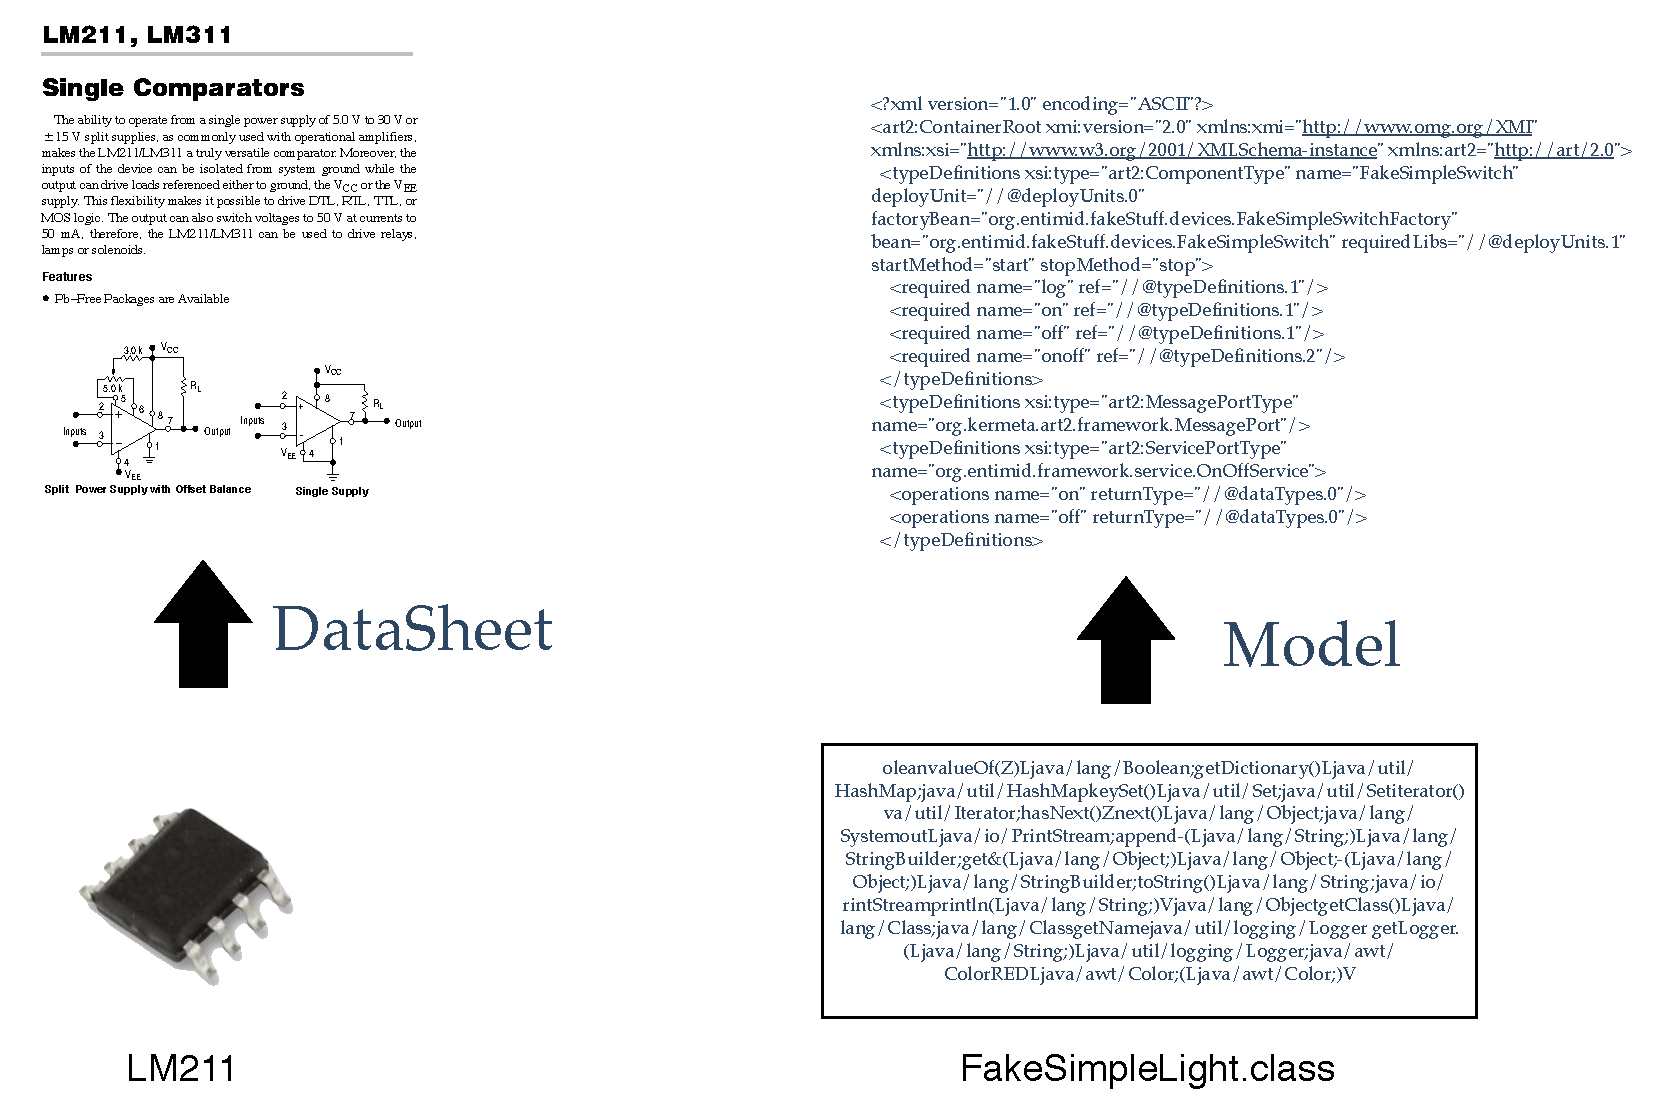
\includegraphics[width=.9\textwidth]{part2/pics/DataSheet.pdf}
	\caption{Electronic Parallel: Datasheets}
 	\label{fig:elecDataSheet}
\end{figure}

The component model created was strongly inspired by electronic components. Indeed, {\it InputPorts} and {\it OutputPorts} have been implemented as presented in figure~\ref{fig:component_type:logical}. They have been divided into \textit{synchronous} and \textit{asynchronous} kinds, to handle both object-based method call handling, and message-based communications between components.\\

\subsection{Meta-Model description}
 
This section details the elements of the component model, presented in~\ref{fig:component_type:model}.\\

{\bf ComponentType}\\

The {\it ComponentType} meta-class carries the component description specification. Ports of the component are describes in collections; provided for input ports, required for output ports. The component type also contains a dictionary which declares parameters, and their default values, that can be specialized for each component instance.\\

{\bf Ports}\\

To keep close to existing component models and promote compatibility, the component model makes use of classical terms in its implementation. As a consequence, {\it InputPorts} are implemented as {\it provided} ports and {\it OutputPorts} as {\it required} ports, as shown in figure~\ref{fig:component_type:model}. For their part {\it ParameterPorts} have been implemented as <key,value> dictionaries.\\

\paragraph{ParameterPorts}
This kind of port is used to specialize component behavior. For example, the \textit{Timer} component uses a \textit{delay} parameter that represents the amount of time to be spent before the time-out occurs. A component can have multiple parameters. They are uniquely named in the component's scope, and can be optional or mandatory. All parameters a component admits are listed in a dictionary at model level.
At runtime, each parameter port is instantiated as a setter method, which only admits a dictionary as parameter. Indeed, each parameter port has its own setter method. Both keys and value types are Strings. This ensures the transmission of parameters in a unified way. Each component is responsible for the conversion from the String to the real type of its parameters.\\
To keep the link with electronic components, the method is the pin, and the dictionary describes the shape of the signal to be sent (voltage, intensity, shape of the signal).

\begin{figure}
\begin{center}
\subfloat[Component Type]{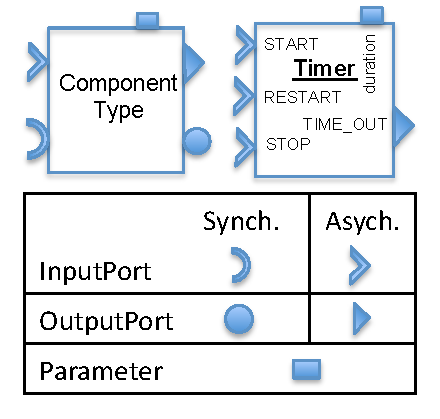
\includegraphics[width=.3\textwidth]{part2/pics/component_type3}\label{fig:component_type:logical}}
\hspace{3mm}
\subfloat[Meta-Model Excerpt]{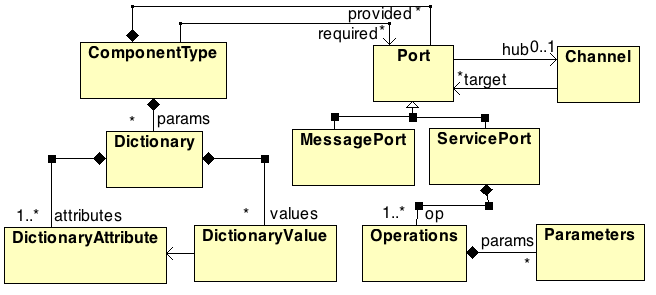
\includegraphics[width=.65\textwidth]{part2/pics/meta-model.png}\label{fig:component_type:model}}
\end{center}
\caption{Extraction of a part of the component model architecture}
\label{fig:component_type}
\end{figure}

\paragraph{InputPorts}
A component can provide several facilities to other components. This is illustrated by the \textit{Timer} on figure~\ref{fig:component_type:logical} which offers start, stop, and restart actions. In classical software component models, the timer component would have provided a single synchronous port with the three start, stop, and restart methods. These methods would have been defined in the StartStopRestart API.\\
Synchronous ports (also called ServicePorts in the model) act the usual way: they are typed by an API, and are based on method calls. Thus, our component model is able to support the common software-component behavior. However, this is not the way of designing components that we encourage.
Indeed, the API is typed by the programming language type system, and this typing may prevent components from being connected because of a mismatch. We want to elevate the typing from the language to the model, and resolve the typing at a higher-level of abstraction.\\
Asynchronous ports, handled as \textit{MessagePorts} in the component model (fig~\ref{fig:component_type:model}), are much more interesting for the promotion of component connectivity. Each method/action a component offers is accessible through a dedicated port. Each port is uniquely named in the scope of the component. In the same way, electronic components have one pin for each action and actions are triggered when the value changes from 0 to 1 for instance, on the corresponding pin.\\
To mimic this behavior, all asynchronous {\it InputPorts} are implemented as a {\it Command} design pattern. They have a unique method {\it public void process(Dictionary<String, String>)}. The uniqueness and standardization of the method are mandatory to ensure the connectivity.\\
Just as an electronic component, actions in our component model can have parameters. Coded in the shape of the input signal passed through an input pin in electronics, our \textit{InputPorts} admit a dictionary of <key, value> parameters. Like ParameterPorts, this dictionary only allows pairs of Strings. These values are specific to each execution and may change form one call to another. In figure~\ref{fig:component_type}, \textit{START}, \textit{STOP} and \textit{RESTART} are all InputPorts. The parameters used on the start or restart activation are transferred through the \textit{TIME\_OUT} OutputPort to the connected component.\\

\begin{figure}
\centering
	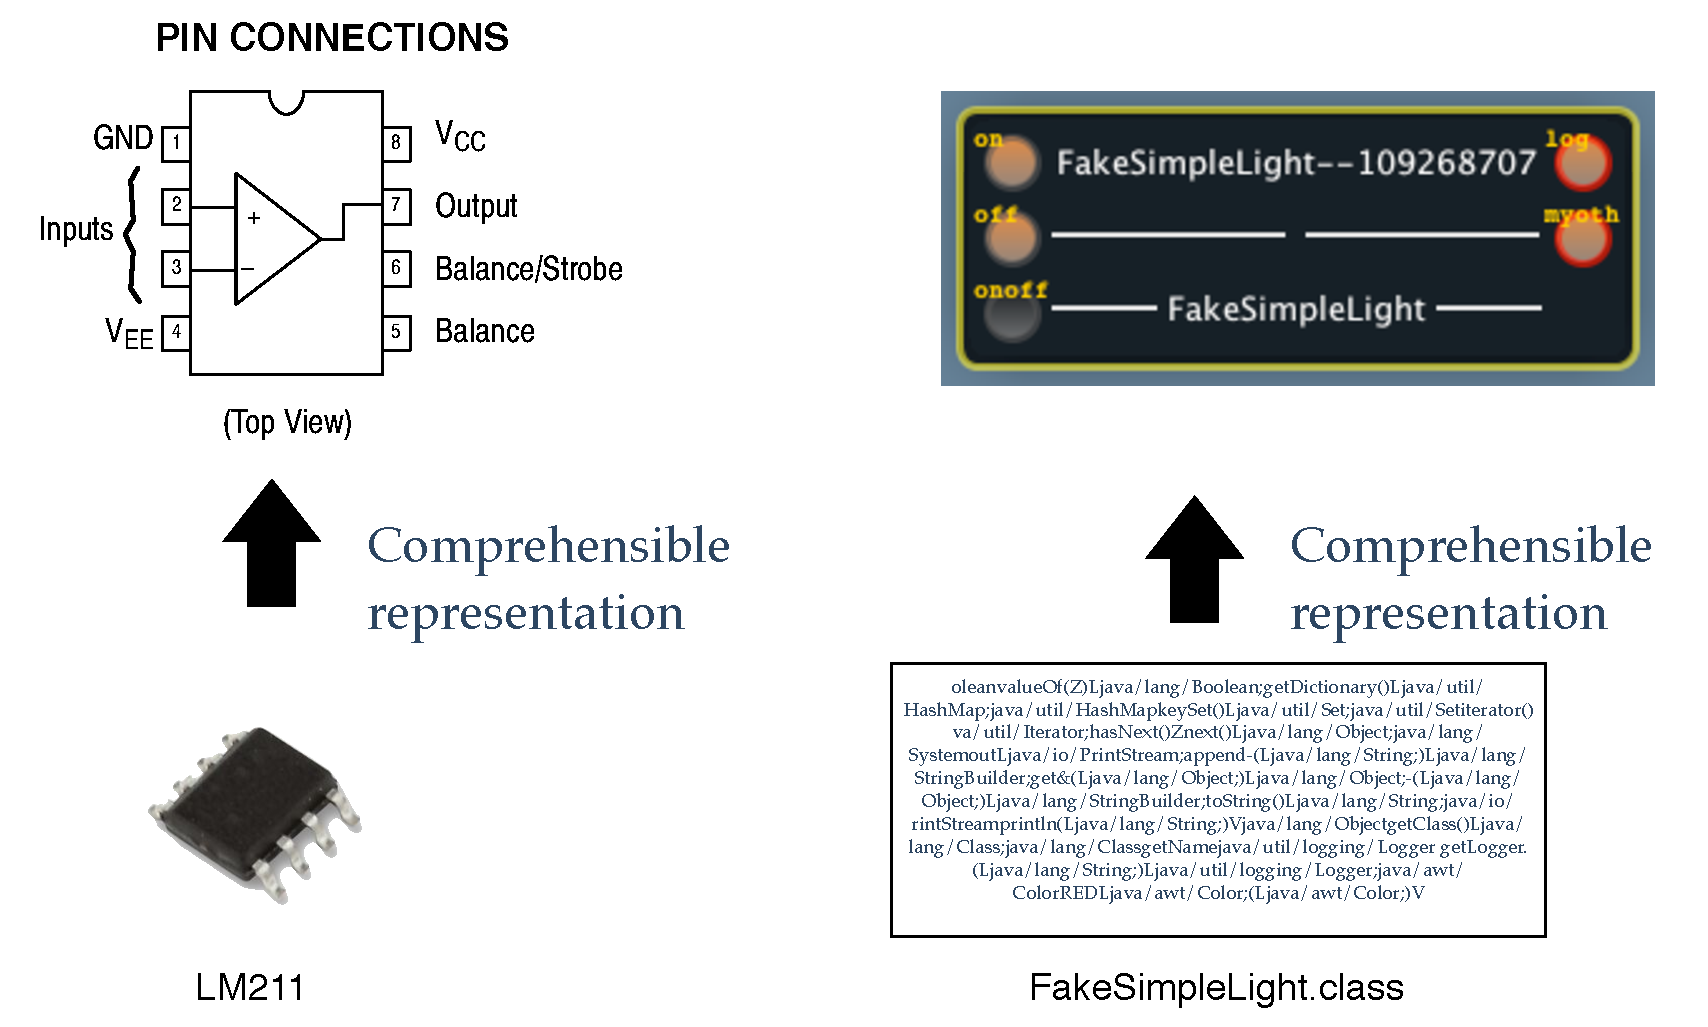
\includegraphics[width=.8\textwidth]{part2/pics/ComponentView.pdf}
	\caption{Electronic Parallel: Components}
  	\label{fig:elecComponent}
\end{figure}


\paragraph{OutputPorts}
The main role of an OutputPort is to forward or release information. For instance, in figure~\ref{fig:component_type:logical} when the timer delay is over, the \textit{TIME\_OUT} port is activated and thus the connected InputPort (if any) also is. In case the activated \textit{InputPort} is synchronous, the result of its activation is returned by the called method. This is a blocking behavior, and may not be adapted to events coming from real life. If the activated port is a MessagePort, the result of its execution (if any) is given though a dedicated \textit{OutputPort}.\\


All this results in a parallel between electronic and software components as shown by figure~\ref{fig:elecComponent}. Input(provided) ports are displayed on the left side, and Output (required) ports are on the right.\\

{\bf Channel}\\

A Channel connects two or several ports. Channels can be of different types, and are instantiated just as components are. Channels are providing communications to components. These communications can be realized with several protocols, politics and media. According to the situation, one can make use of a channel that sends messages in sequence, or of one sending in parallel. Channels can create the link using TCP or UDP sockets, RS232 serial connection, or a REST request. Channels are handling the communication semantic and method between components.\\
Being defined outside the component, developers can make no assumption about the media or protocol that will be used, or the kind of component on the other side. This enforces the development of well defined standalone components and promote their reuse.\\

{\bf Service Ports}\\

Service ports come with the description of their operations (name, returned value) and a description of the operations' parameters (names and types). These information are used by channels, modeling tools and runtime platforms. Channels can play a role of mediation between not exactly aligned services descriptions. Modeling tools use these description to perform checks on component assemblies and authorize au not components' connections. Finally, runtime platforms can check the alignment, and may refuse any connection that violates a pre-defined connection rule.\\
These checks are detailed in section~\ref{subsec:check_to_validate}.

\subsection{Concrete example}
\label{subsec:compoModConcreteExample}
This example shows how a real product is implemented in this component model. The RMG4S, on the left side of figure~\ref{fig:rmg4s}, is a KNX product by Theben\footnote{http://www.theben.de/en}. This product can control up to four 230V lights or sockets. Its virtual representative has 8 message input ports, two (i.e.: on, off) for each controllable element. When a physical event changes the state of an output of the product (somebody switches on the light using the dedicated switch), the state is propagated to any connected device, through the corresponding port of the component.\\
In addition, a {\it KnxEnv} input port allows the driver to circulate real-life events. On the other hand, an output port {\it KnxNetwork} is used to send events from the model element to the real product through the driver. The last output port is a logging port.\\
Thus, to switch on the light that is physically connected to the first module of this product, one just has to activate the {\it m1\_on} port. The component then asks its driver to send a message to the real device to make it power up its first module.\\
On the other hand, when the state of a module is physically changed, a message is sent from the driver to the component. The component then activates the {\it m1\_state} (for instance), to inform any connected component about the change.\\
If the application proposes a graphical user interface, the {\it on} (resp. {\it off}) port of the component is activated when the user presses the graphical button. On activation, the driver sends the order to the real product, which reacts and sends information about its state change. The driver catches the information, and sends it to the graphical interface for update, through the dedicated output port of the component.\\ 

\begin{figure}
\centering
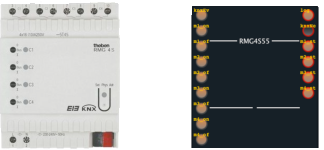
\includegraphics[width=.7\textwidth]{part2/pics/RMG4sModel}
\caption{Example Model}
\label{fig:rmg4s}
\end{figure}

The component model makes our software equivalent to electronic components \textit{DataSheets}. Assembly constraints, mandatory parameters on ports, component behavior, and many other pieces of information on components can be expressed in the model. This abstract description of the component has no effect on the runtime implementation (just as \textit{DataSheets} have no effect on black-box components by the way).\\


\subsection{Implementation and Model Relationship}
\label{subsec:compModBinToModel}
\begin{figure}
\centering
\begin{lstlisting}[caption=Java class POJO annotation,label=fig:jcPOJOannot,basicstyle=\scriptsize\ttfamily,tabsize=2 ]
@Provides({
    @ProvidedPort(name = "start", type = PortType.MESSAGE),
    @ProvidedPort(name = "stop", type = PortType.MESSAGE),
    @ProvidedPort(name = "restart", type = PortType.MESSAGE) })
@Requires({
    @RequiredPort(name = "timeOut", type = PortType.MESSAGE),
    @RequiredPort(name = "logger", type = PortType.MESSAGE) })
@DictionaryType({
    @DictionaryAttribute(name = "time", default="3000") })
@Library(name="EnTiMid - Framework")
@ComponentType
public class Timer extends AbstractComponent {

	private TimerThread timer;
	private long time = 3000;  // default value

	public Timer() {}
	public Timer(final long time) { this();  this.time = time; }

	public long getTimeOut() { return this.time; }    
	public void setTimeOut(long value) {
		if (value > 0) { this.time = value; }
	}

	@Port(name = "stop")
	public void stopTimer(Message m) {
		if (timer != null) { timer.reset(); }
		getPortByName("logger", MessagePort.class).process("Timer("+time+")::STOP");
	}

	@Ports({ @Port(name = "restart"), @Port(name = "start") })
	public void restartTimer(Message m) {
		if (timer != null) { timer.reset(); }
		timer = new TimerThread();
		timer.start();
		getPortByName("logger", MessagePort.class)
			.process("Timer("+time+")::STARTED");
	}

	@Start
	public void start() {
		time = Integer.valueOf(getDictionary().getValue("time")).intValue();
		getPortByName("logger", MessagePort.class).process("Start Timer");
	}

	@Stop
	public void stop() {
		getPortByName("logger", MessagePort.class).process("Stop Timer");
	}

	@Update
	public void kevUpdate() {
		time = Integer.valueOf(getDictionary().getValue("time")).intValue();
		getPortByName("logger", MessagePort.class).process("Updating Timer");
	}
\end{lstlisting} 
\end{figure}


The development of a component (i.e.: a virtual representative of a physical device) can be achieved in two ways. According to its preferences, the developer can make the model of what he wants, and ask for code generation. This approach is called {\it Model First}. The model can also be extracted directly from annotations decorating the implementation code made by the developer. This is called {\it Code First}. The code first approach differs from a reverse engineering approach, in the sense that the model is extracted from annotations in the code, and not from the implementation code itself. These two approaches are not exclusive. The model of a component can evolve, therefore impacting its implementation. Respectively, if a change is made to the code, it has to be reproduced at the modeling level. In other words, the consistency between implementation and model has to be guaranteed.\\

To illustrate the description, listing~\ref{fig:jcPOJOannot} shows the complete implementation class of a {\it Timer} component. This listing is organized as follows: on the first lines are annotations on the class that describe the component shape. Just after, the class definition comes with private attributes, object builders, then getters and setters. Next, methods render the services offered by the component. Life-cycle management methods are at the end of the class.\\

{\bf Component shape}\\
The first annotations on the class inform about the {\it Input}, {\it Output} and {\it Parameter} ports. As explained in section~\ref{subsec:makeSoftCloserToElec}, {\it InputPorts} are implemented as {\it provided ports}. Common actions that can be carried out on a timer (start, stop, restart) are listed under these terms.\\
This {\it Timer} implementation offers two outputs, visible as {\it Required Ports}. A {\it log} port, which sends information about the internal behavior of the component, and a {\it time\_out} port activated when the countdown ends.\\
The Timer admits a parameter. This parameter sets the delay between the start and the activation of the time\_out port. This parameter appears in a dictionary.\\
The {\it @Library} indicates that the component is part of the virtual library of components called "EnTiMid - Framework". In edition tools, all components of the same library are presented under the same package of components. A library of components can be defined using several deployment units.\\
The last annotation tags the class as a component type implementation. This annotation is mandatory for the compilation tools to consider the class as a component type.\\

{\bf Port mappings}\\
Once described, input ports have to be linked to the method implementing the action. In the example, one may remark that a port can be bound to at most one method, but a method can be reached from several ports (1 method can be mapped on n ports). Indeed, the behavior of a {\it start} and a {\it restart} of a timer are implemented the same way. Classical solutions could have been to remove one action or to copy-paste the method. From a user perspective (sect.~\ref{subsec:keepUserInMind}), a Timer should be able to be started and restarted which implies not to removing the port. Thanks to this multiple mapping, the user will be satisfied with no redundancy of code.\\
Moreover, the transfer of the annotation from one method to another, changes the method called when a port is activated. This change is completely transparent for assemblies already using the component, since the annotation is not modified. This is a great ability that enables changes in the implementation and method names, with no change in the component interface.\\
Finally, a component can offer the same service through both {\it Service} and {\it Message} port. Using the same mechanism, the same method can be called in both cases.\\

{\bf Life cycle}\\
{\it Start} and {\it Stop} life cycle methods are mandatory. They are called when an instance is started (resp. stopped). Stateless components may just ignore these methods, but stateful ones may use these to persist their state.\\
The {\it update} method is used to inform a component that one of its parameters has changed.\\

{\bf Code first}\\
Meta-information, concerning the component model, is introduced in the code using annotations. This method for including meta-information in the code has already been used in tools such as Fraclet\cite{Rouvoy:2009}. A developer familiar with the annotation set, or in charge of the migration of existing components, may directly define the model in the code.\\
As in a classical development process, the new implementation code has to be compiled to incorporate the changes in binaries. Our component model takes advantage of the compilation phase to extract the model from the annotations. A visitor goes all over compiled classes and selects the {\it @ComponentType} decorated classes. Then sub-visitors navigate into the code to create the model.\\
At the end of the compilation process, the newly-computed model is added into the compilation result. {\it i.e.} the model is included as an XML file into the {\it .jar} that results from the compilation. Model consistency with the latest code version is guaranteed this way.\\

{\bf Model First}\\
Writing component type code, plus the annotations, may become a complicated task. A non-familiarized person may experience difficulties in placing all the annotations required to describe its component.
The model-first approach aims at providing tools to graphically (or textually) describe the component first, and then ask for the implementation to be generated. This method is made available by the use of tools such as graphical \gls{dsl}, textual \gls{dsl} or generic meta-modeling languages such as Kermeta~\cite{Muller05a}. Models bring a more intuitive approach for the description of a component.\\ 
Once the developer is done with its component's model, the generation tool is activated. If the implementation class of the component does not already exist, a new file is created. This file contains the skeleton of the component implementation. The code generation reaches its limits when the body of methods has to be created. The behavior of methods is the only part to be completed by hand by the developer. Otherwise, the class is already decorated with all annotations, and ports are mapped by default on generated methods.\\
When an implementation class already exists, the generation process is slightly more complex. In fact, a temporary model is extracted from the existing code and an \gls{ast} of the code is created. The \gls{ast} describes the code using a tree structure containing objects. Each object stands for a method, an argument, an attribute, etc. A comparison is made between the model created by the user, and the model extracted from the existing code. Each difference is analyzed, and modifications are made on the \gls{ast}. The final code is generated from the modified \gls{ast}.\\
The model-first approach helps somewhat in linking the model and the code. In any case, the resulting code still needs a developer to complete the new methods created, to remove dead code and to optimize the mappings.\\

Thanks to these mechanisms, models of components are available while the system is not running. Their conformance with the actual implementation is guaranteed by construction. This model abstraction makes it possible to create and exploit tools from \gls{mde}.\\


\subsection{Implementation independence}
\label{subsec:compImplIndep}

As previously presented, the model of a component is independent from the actual implementation. Listing ~\ref{fig:implIndep} illustrates this independence. Indeed, the FakeSimpleLight component declares a {\it onoff} provided port that renders a OnOffService. The OnOffService class is a Java interface containing two methods {\it on} and {\it off}, a kind of contract the component ensures this port is compliant with. However, the implementation class of the component does not actually implements the interface.\\
\begin{figure}[h!]
\centering
\begin{lstlisting}[caption=Implementation independence,label=fig:implIndep,basicstyle=\scriptsize\ttfamily,tabsize=2 ]
@Provides({
    @ProvidedPort(name = "on", type = PortType.MESSAGE),
    @ProvidedPort(name = "off", type = PortType.MESSAGE),
    @ProvidedPort(name = "onoff", className = OnOffService.class)
})
@ComponentType
public class FakeSimpleLight extends AbstractFakeStuffComponent {
 @Ports({
  @Port(name = "on", method = "process"),
  @Port(name = "onoff", method = "on")})
 public void lightOn(Object o) {
  [...]
 }

 @Ports({
  @Port(name = "off", method = "process"),
  @Port(name = "onoff", method = "off")})
 public void lightOff(Object o) {
  [...]
 }
 [...]
}
\end{lstlisting} 
\end{figure}\\
Each method of the OnOffService is bind on a method of the component's implementation by mean of a {\it Port} annotation. Since the component does not implement the OnOffService interface, the Java compiler can not check that all methods are present. This check is thus performed while parsing the annotations for the extraction of the model, before the actual compilation.



\subsection{Link with the interoperability layer}
\label{subsec:compModLinkWithInterop}
The actual implementation of the component model is slightly different from the view developers can have of components. The connection between two components(channel) is graphically a line linking two ports (see the top of figure~\ref{fig:linkWithInteropLayer}). The line represent a channel, dependent of the channel type selected in the library at design time. Since ports can be synchronous or asynchronous, the runtime cannot handle port connections in the same way. The activation of an output port implies different behaviors according to its type. A message output port will send messages on topics to activate the linked input ports, but a service port has to start a method call.\\

\begin{figure}[h!]
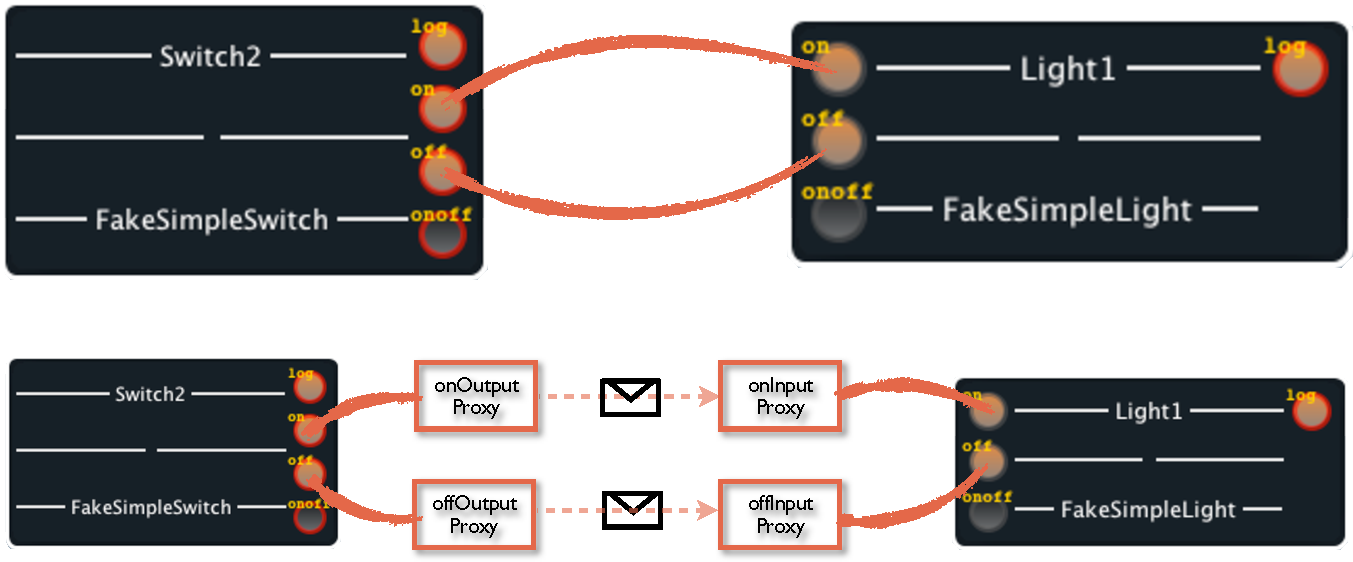
\includegraphics[width=\textwidth]{part2/pics/InteropModelLink}
\caption{Link between the interoperability layer and component connections}
\label{fig:linkWithInteropLayer}
\end{figure}

This complexity is hidden from developers in both the code and the model view of the components, by the use of proxies behind the concept of channels. At runtime, a proxy is generated for each port connected to another component's port, as illustrated in the bottom of figure~\ref{fig:linkWithInteropLayer}.\\
If the port is a message port, the proxies use messages and topics to communicate with each other. When an output port is activated, its proxy generates and sends a message on a pre-defined topic. On the other hand, a proxy listens to this topic only, and activates the input port on which it is connected when a message arrives. Activations are carried out with a {\it Command} design pattern, from the output port to activate the proxy, and from the proxy to the input port. The mechanism is thus transparent from the developer's viewpoint: an input port must provide a command pattern, an output port activates a command pattern.\\

The mechanism of proxies has also been implemented to handle the method calls of service ports. Links between components' ports are thus handled in a uniform way. The introduction of proxies makes it possible to use other means of communication (in the case of distribution issues for instance), and enables some adaptation mechanisms.\\

\subsection{Main advantage of this component model}

The main advantage of this component model is the location of the type checking. The typing of components was completely relaxed in the implementation to eliminate interoperability problems due to the implementation language type system. The typing was moved to the model level, where checks and changes in rules are made much simpler. This contribution paves the way for a pluggable type system~\cite{PapiACPE2008,Bracha:2004}.\\


\subsection{Summary}

This new component model answers the need for a tool to make the abilities of devices and their interactions explicit at design runtime. Annotations in the code is a convenient way to integrate the component model into the implementation code, and ensure the synchronization between the model and the implementation. The component model also eases the reading and understanding of an application, since all links between components are made explicit.\\

The component model imposes that the configuration is completely defined, but it is not responsible for its deployment. A gap from the component assembly to the sequence of commands to set up the application at runtime still has to be filled.\\
Since the component model has been made flexible to allow all possible connections, any connection is possible, but some may not be desirable. Just as in electronics, assemblies are constrained by components' specificities. If electronic boards allow all possible connections, components have constraints to be respected in order to assert their behavior. Assemblies have to be verified and simulated, to prevent any undesirable interactions.\\

To eliminate these two issues, the Model@Runtime approach and model checkers have been used in \enti{}. Model checkers enable verifications of component assemblies at several steps of the development, while the model@runtime takes responsibility for bridging runtime elements and the component model. These two elements of the proposal make the {\it Model@Runtime and Reasoning Engine} layer.\\


\section{Model@Runtime and Reasoning Engine}
\label{sec:martAndReasoning}

\begin{wrapfigure}{r}{60mm}
  \vspace{-5mm}
  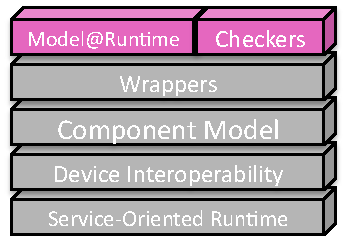
\includegraphics[width=60mm]{part2/pics/layers/MartReasoners.pdf}
%  \caption{Modeling Layer}
%  \label{fig:modelingLayer}
  \vspace{-5mm}
\end{wrapfigure}

The {\it Component Model} layer provides a level of abstraction from the implementation specificities. It offers a unified model view of components and their constraints and enables the creation of management tools. Reasoning engines, checkers, and models@runtime abilities can be used to ease the creation of component-based applications.\\
The first requirement targets the validation of assemblies, prior to their real deployment. This checking step is described in section~\ref{subsec:check_to_validate}. Section~\ref{subsec:modelatruntime} presents an overview of the use made of Models@Runtime techniques in this approach.

\begin{figure}[h!]
	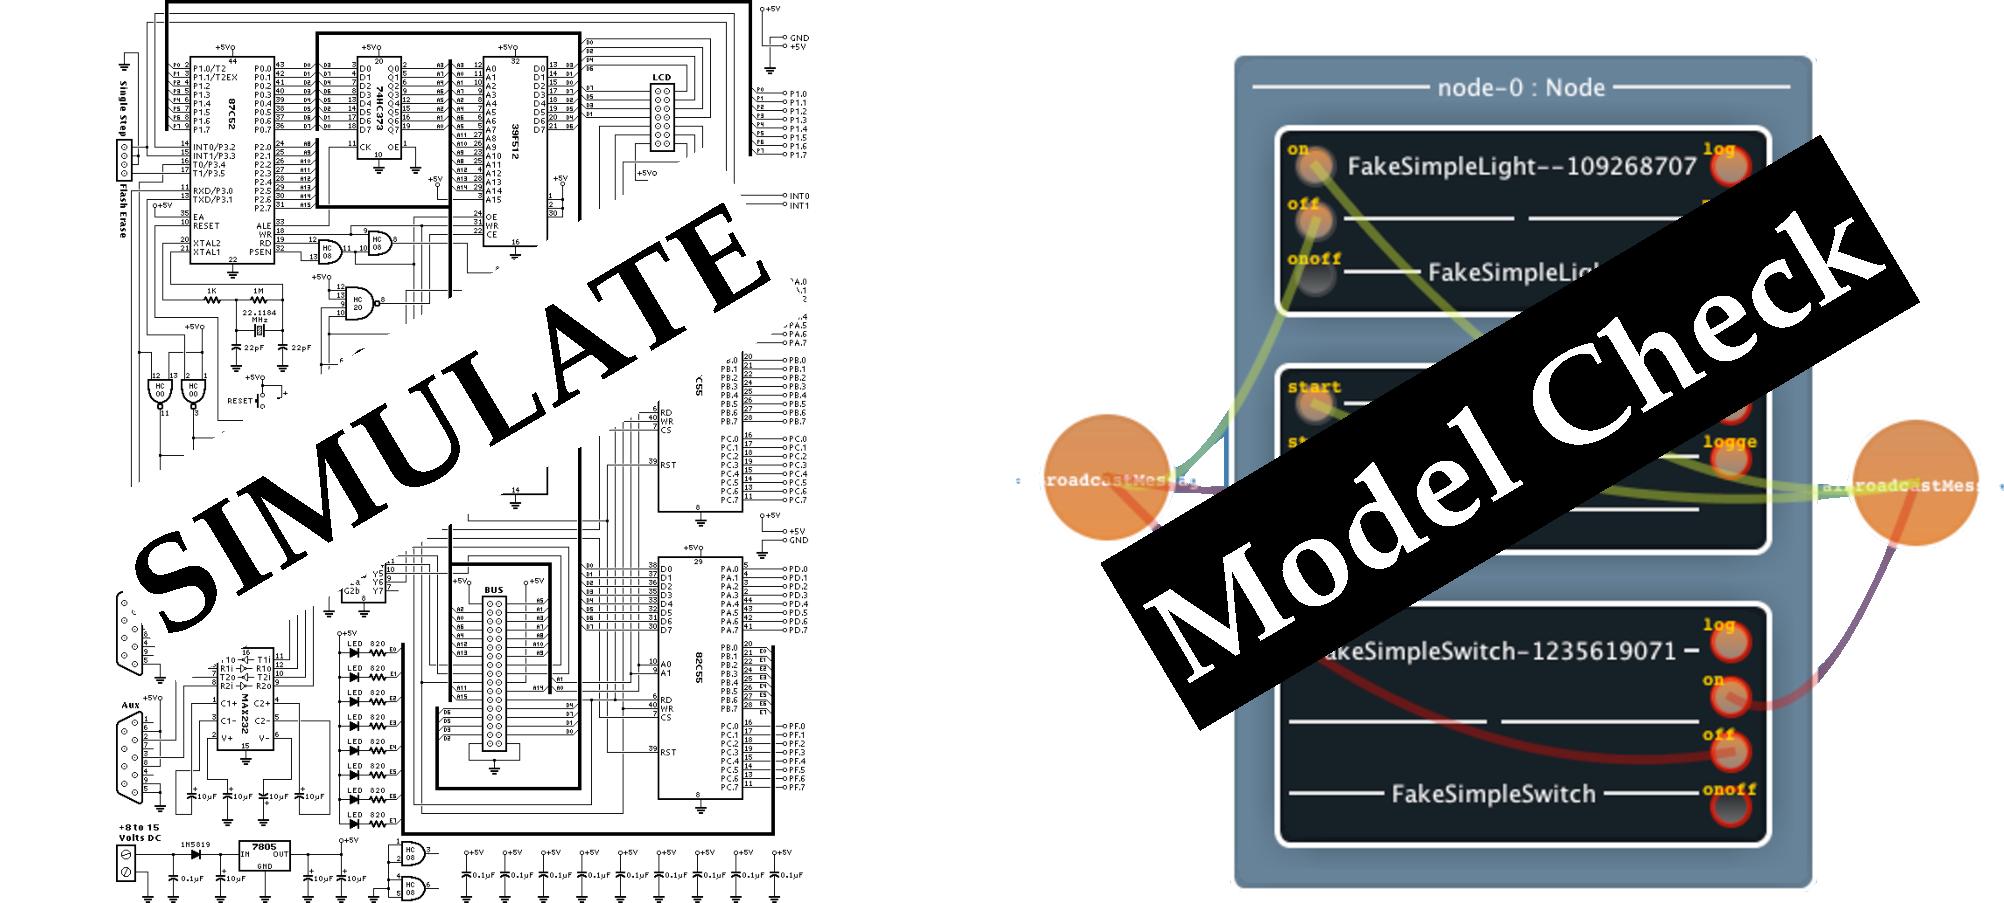
\includegraphics[width=\textwidth]{part2/pics/ModelCheck.pdf}
	\caption{Electronic Parallel: Simulation}
  	\label{fig:elecSimulation}
\end{figure}

\subsection{Check to validate}
\label{subsec:check_to_validate}

In electronics, the components' assembly has to be approved. Its conformance in relation to components and applications-specific constraints has to be guaranteed. This validation prevents assemblies from having any computable damage. This conformance check is often carried out by simulations, based on components' specifications described in their documentation. Figure~\ref{fig:elecSimulation} shows once again the parallel between the electronic approach and ours, where electronic simulations are replaced by model checking in our context.\\

\begin{figure}[h!]
\centering
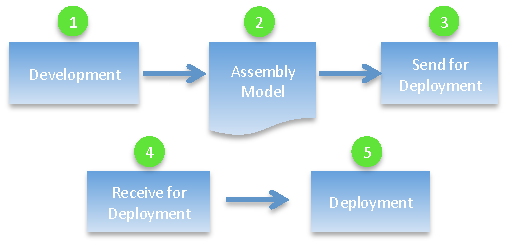
\includegraphics[width=.8\textwidth]{part2/pics/CheckPositions.pdf}
\caption{Checkpoint positions in the assembly deployment chain}
\label{fig:checkPoints}
\end{figure}



In a classical software engineering process, conformance checking is done at 1) design time by the developer, 2) compilation time automatically, and 3) by running tests on the application built. The modeling approach offers a way to perform more precise checks, targeting more specific concerns, at several moments between the design and deployment phases.\\
Checking methods presented here have been written in Kermeta~\cite{Muller05a}. Kermeta is a modeling and aspect oriented programming language. Its underlying metamodel conforms to the EMOF standard. It is designed to write programs which are also models, to write transformations of models (programs that transform a model into another), to write constraints on these models, and to execute them. Once written, there rules have been compiled and integrated in the model editor and in the runtime platform.\\
Figure~\ref{fig:checkPoints} displays the different moments where checks can be performed and illustrates what can be checked at each moment. These steps are detailed in the following paragraphs.

\vspace{0.75cm}
\begin{enumerate}
\item {\bf Developer's actions}\\
The assembly tool can monitor developers' actions. During the design phase, checkers can verify that only authorized operations are executed by the developer. When an inappropriate action is carried out, the triggering of warnings and errors can improve the development process. Thanks to this information, developers can immediately correct their code and learn from their mistakes. The earlier errors are detected and corrections made, the more the impact on the global solution is reduced. Also, developers' profiles could be created and associated with different checking policies according to the developers' expertise. This provides a fine-grained checking process for the design of applications.\\
Listing~\ref{fig:checkDevAct} illustrates this by checking that for each channel, all connected ports are of type Service, or Message, but not both.

\begin{figure}[h!]
\centering
\begin{lstlisting}[caption=Example checking developpers' actions,label=fig:checkDevAct,basicstyle=\scriptsize\ttfamily,tabsize=1 ]
operation checkBindingsHomogeneity(model:ContainerRoot)
	: Sequence<CheckerViolation> is do
 var violations : Sequence<CheckerViolation>
 model.hubs.each { channel |
  var bindingsOnChannel : Sequence<MBinding>
  bindingsOnChannel := model.mBindings.select{mb |
   mb.hub.equals(channel)
  }
  var synchBindings :  Sequence<MBinding> 
  var asynchBindings : Sequence<MBinding>
  bindingsOnChannel.each { binding | 			
   if binding.port.portTypeRef.isKindOf(ServicePortType) then
     synchBindings.add(binding)
   else
     asynchBindings.add(binding)
   end
  }
  if (not synchBindings.isEmpty) and (not asynchBindings.isEmpty) then
    var violation : CheckerViolation init CheckerViolation.new
    violation.message :=
    "Ports of both Service and Message kinds are connected to the same channel:"
    + channel.name
    violations.add(violation)
   end  			
 }
 		
 result := violations
end
\end{lstlisting}
\vspace{-0,4cm}
\end{figure}

\vspace{0.50cm}

\item {\bf Assembly constraints}\\
The structure of an assembly can be constrained by rules, due to runtime constraints, or due to the framework used. These rules are neither specific to the developer, nor to the targeted business. A general policy could impose assemblies to be composed with at least two communication components. This constraint aims at keeping continuity in the communication service in case of failure. Valuable for all applications created by the company, this rule is shared by all software development projects.\\
The method presented in Listing~\ref{fig:checkAssembly} checks that for each component instance, all mandatory ports are connected to a channel.

\begin{figure}[h!]
\centering
\begin{lstlisting}[caption=Example checking assembly constraints,label=fig:checkAssembly,basicstyle=\scriptsize\ttfamily,tabsize=1 ]
operation checkMandatoryConnections(model: ContainerRoot, node : ContainerNode)
	: Sequence<CheckerViolation> is do
 var violations : Sequence<CheckerViolation>
 node.components.each { component |
  component.required.each { port |
   if( not port.portTypeRef.optional) and port.isBind then
     var concreteViolation : CheckerViolation init CheckerViolation.new
    	 concreteViolation.message :=
      "Required port (" + port.eContainer.asType(ComponentInstance).name
      + "." + port.portTypeRef.name
      + ") is not bind"
    	 concreteViolation.addTargetObject(port)
    	 violations.add(concreteViolation)
   end
  }
 }
 result := violations
end
\end{lstlisting} 
\vspace{-0,3cm}
\end{figure}

%\vspace{1cm}

\item {\bf Business Rules}\\
An application created to control a plane has different constraints compared to a watering management system. Each application domain can require that special rules are considered. This checkpoint is placed just before the model deployment. The validation of conformance at this moment avoids the sending of corrupted models to the runtime.\\
The rule presented in Listing~\ref{fig:checkBusiness} verifies that for each channel, all connected ports have the same name.

\begin{figure}[h!]
\vspace{-0,3cm}
\centering
\begin{lstlisting}[caption=Example checking identical port names,label=fig:checkBusiness,basicstyle=\scriptsize\ttfamily,tabsize=1 ]
operation checkPortsEquality(model:ContainerRoot)
	: Sequence<CheckerViolation> is do
 var violations : Sequence<CheckerViolation>
 model.hubs.each { channel |
  var bindingsOnChannel : Sequence<MBinding>
  bindingsOnChannel := model.mBindings.select{ mb |
   mb.hub.equals(channel)
  }
  var portName : String init ""
  bindingsOnChannel.each { binding |
   if portName.equals("") then
     portName := binding.port.portTypeRef.name
   else 
    if not binding.port.portTypeRef.name.equals(portName) then 
      var violation : CheckerViolation init CheckerViolation.new
      violation.message := "Connection not authorized."
	  violations.add(violation)
    end
   end
  }
 }
 result := violations
end
\end{lstlisting} 
\vspace{-0,4cm}
\end{figure}

\item {\bf Platform Rules}\\
A platform is a system composed of both software and hardware. The composition of the execution platform may impact the development, or deployment of a component-based application. The role of this check is to verify that all constraints inherent to the platform choice are respected. As checks are performed at the model level, they can be realized by the runtime platform itself, with no consequence on the running application. For instance, a model can be rejected if one of the components requires a serial connection, and the runtime hardware of the platform has none.\\
The Listing~\ref{fig:platformChecks} ensures no channel is using the SerialConnectionChannel, probably because the hardware does not have any serial port. Modeling the platform resources could enable to move these checks to before deployment and thus gain time.

\begin{figure}[h!]
\centering
\begin{lstlisting}[caption=Example checking pre-deploy constraints,label=fig:platformChecks,basicstyle=\scriptsize\ttfamily,tabsize=1 ]
operation serialConnectionCheck(model:ContainerRoot)
	: java::lang::util::List<CheckerViolation> is do
 if model.getChannels.exists { channel |
 	channel instanceOf SerialConnectionChannel
 }.isEmpty then
   var concreteViolation: CheckerViolation init CheckerViolation.new
   concreteViolation.setMessage(
    "SerialConnection not supported. (" + channel.getName + ")"
   )
   concreteViolation.setTargetObjects(channel)
   violations.add(concreteViolation)
  end
  result := violations
end
\end{lstlisting} 
\vspace{-0,3cm}
\end{figure}

\item {\bf Check deployment commands}\\
If the model of the assembly successfully passes all checkpoints, it is ready for deployment. The last step of checking consists in the first step of Models@Runtime mechanisms. The deployment of a component assembly is split into several commands. This last verification ensures that all commands are executable before running the sequence. This phase is handled by the Models@Runtime engine. Its job consists in (1) defining the best way to go from the current system assembly to the new assembly received, and (2) supervising the migration. This is explained in section~\ref{subsec:modelatruntime}.

 
\end{enumerate}



\subsection{The Model@Runtime engine work}
\label{subsec:modelatruntime}
In his PhD Thesis~\cite{Morin:2010}, Morin presented the concepts of a Model@Runtime engine. The Model@Runtime engine is responsible for several actions. First of all, it has to constantly maintain a model view of the running system. Secondly, when a new model is asked to be deployed, the Model@Runtime engine plans the migration (i.e.: identifies and sequences the necessary primitive commands). Lastly, it supervises the run of the migration command sequence, in order to roll back to the previous stable state in case of failure.\\
The next paragraphs provide an overview of the engine work, in order to ease the comprehension of solution in its entirety.\\

{\bf Identify and validate the changes} \\
After validation, the first task is to identify the differences between the model representing the running system (source model) and the target model the system must switch to, as illustrated in figure~\ref{figure:comparison}. During the comparison, the next 7 types of primitive commands can be found. \textit{1.} {\bf start} and {\bf stop} components. \textit{2.} {\bf add} and {\bf remove} components. \textit{3.} {\bf add} and {\bf remove} bindings. \textit{4.} {\bf update} components.
\begin{figure}
\begin{center}
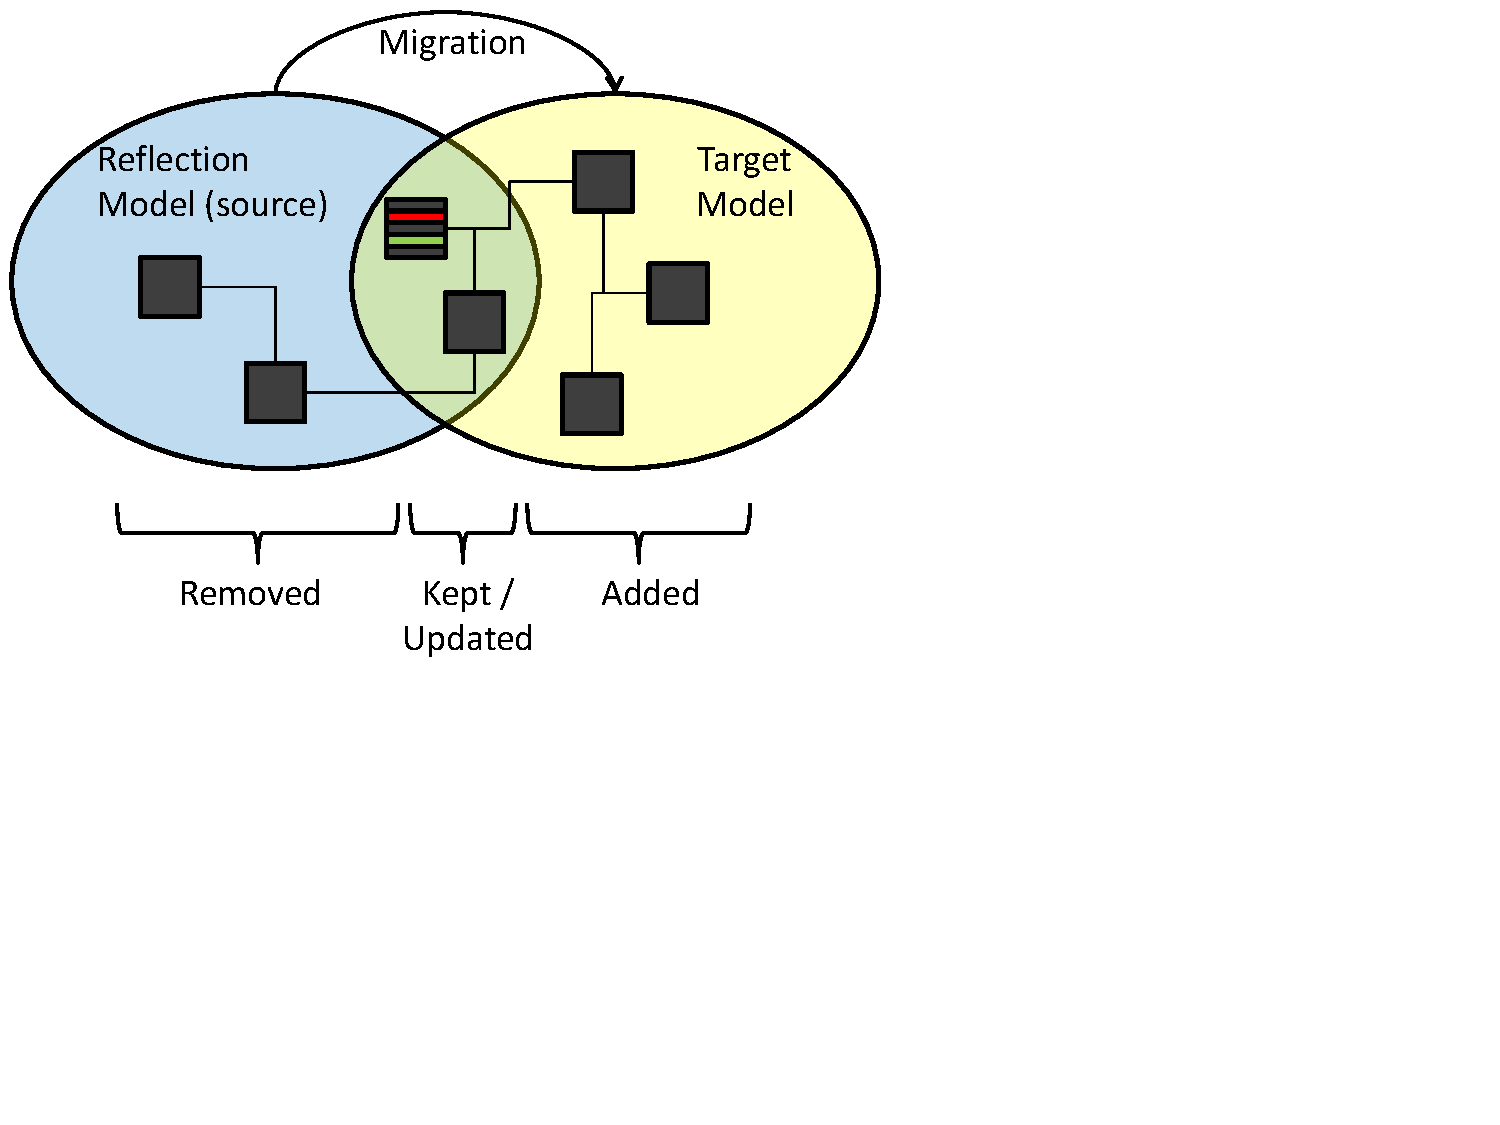
\includegraphics[width=7cm]{part2/pics/comparison}
\caption{\label{figure:comparison} Identifying differences between the source and the target configurations.}
\end{center}
\end{figure}
The steps to go from the current configuration to the required one are specified by primitive commands that represent atomic differences between the two configuration models.
The comparison system only deals with abstract commands, to allow a change of the component management policy. The real commands are instantiated (not yet executed) according to the actual policy, during the model comparison.\\

{\bf Planning the execution sequence}\\
These commands are stored in a collection and ordered according to a heuristic~\cite{Andre:2010,Bratskas:2010} that ensures a safe migration from the current to the target configuration. Before actually executing the commands, the list is parsed to verify that all the commands can be executed. For example, for all {\it AddComponent} commands, the presence of the specific component factory is checked, to ensure all components can actually be added without any problems. Doing this kind of verification for all commands ensures that the command execution will execute properly. If a command is detected as non-executable, a report clearly describes the problem, and no command at all is executed. This way, the system is always kept consistent.\\

{\bf Roll-back abilities}
In case the migration fails, each command is decorated with a roll-back equivalent command. Thus, each command executed before the failure can be cancelled. Moreover, a second protection in place consists in keeping the old model in memory. If everything goes wrong, it is always possible to restart from scratch, and migrate back to the old model.\\

{\bf Specificities of components and services}\\
Because of an adaptation, some links (bindings) between components may appear or disappear, for the system to act differently. In the case of classic components, adding or removing bindings is realized by setting or unsetting a variable. Generally, a component missing one mandatory binding is stopped, because it cannot run any longer. However, in the case of service-based systems such as \enti{}, the component may still offer its services to third-party applications, and thus, should not always be stopped. In other words, a "light component", a virtual representation of a real light, may not be bound to any other component, but might still serve another application for the control of this light.\\
Other behavioral constraints can require more complex actions than just a set or an unset. For instance, if an alarm has been triggered and if the user does not process this alarm, the system must be able to propagate the information somewhere else for the alarm to be treated. The removal of a communication link is structurally correct, but the link may take part in an operation being treated, and so, it has to be kept until the end of the action.\\

As previously explained, real commands for the migration are instantiated according to the current policy of the running system. Real commands can also be specialized for each runtime they have to be applied on. In our context, atomic commands have been instantiated to address a service-oriented runtime. Indeed, this runtime has offered all the facilities required by our approach. This is detailed in section~\ref{sec:soaruntime}.

\newpage
\section{Service-Oriented Runtime Architecture}
\label{sec:soaruntime}

\begin{wrapfigure}{r}{60mm}
  \vspace{-5mm}
  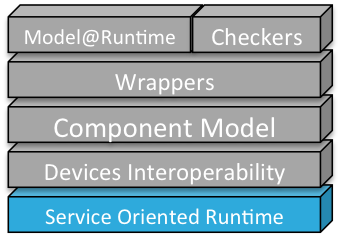
\includegraphics[width=60mm]{part2/pics/layers/SoaRt}
%  \caption{Service Oriented Runtime}
%  \label{fig:soaLayer}
  \vspace{-5mm}
\end{wrapfigure}

For the proposed approach to efficiently cope with dynamic evolutions, the underlying runtime environment is required to offer dynamic abilities. As explained in~\cite{Di-Nitto:2008}, the concept of service has emerged as a good candidate to cope with the dynamicity of adaptive systems. The adoption of this concept led to the development of technologies, standards, and methods to build service-based applications. Since the Service-Oriented paradigm insists on the pervasiveness of services, it imposes service-based applications to properly handle this requirement. Indeed, services can appear and disappear at any time, and applications built upon these principles have to take these constraints into account.\\

The OSGi Alliance~\cite{OSGI:r4}, a 'consortium of technology innovators', has released a set of specifications that define a service-oriented platform, and its common services. This Service-Oriented Runtime has been selected to support commands that require adding or removing component instances and types(binaries), during the execution.\\

{\bf Dynamicity in OSGi}\\
The OSGi kernel is a standard container-provider to build service-oriented software systems. It implements a cooperative model where applications can dynamically discover and use services, provided by other applications running inside the same kernel. It provides a continuous computing environment. Applications can be installed, started, stopped, updated, and uninstalled, without a system restart. It offers a remote management model for applications that can operate unattended or under the control of a platform operator. Finally it embeds an extensive security model, so that applications can run in a shielded environment. According to these specifications, an application is then divided into several bundles. A bundle is a library component in OSGi terms. It packages services that are logically related. It imports and exports Java packages, and offers or requires services. Services are implementations of Java interfaces.\\

{\bf Modularity}\\
Each OSGi bundle is designed to reach the highest level of independence, giving the software enough modularity to allow partial service updates, additions or removals. This programming style allows software-builders to deploy the same pieces of software for all of their clients, either professionals or private individuals and then simply adapt the services installed. Moreover, the services running on the system can be changed during execution.\\

\vspace{0.5cm}
{\bf Component Types, Instances and Bundles}\\
Described in section~\ref{subsec:modelatruntime}, the Model@Runtime engine creates an ordered sequence of commands when it receives a new model to deploy. Each command of the list is then translated into an OSGi command.\\
In \enti{}, component types are contained in OSGi bundles. These bundles are only used as deployment units and do not provide any service. They just embed components. When an {\bf addComponent} command is parsed, the runtime checks if the component type is available in the environment. If not, the bundle containing the type is downloaded and installed. Once the component type is available, a new instance can be created.\\
Component instances are also mapped on bundles because of their independent life-cycle management. Indeed, {\bf start} or {\bf stop component} commands are directly translated to start and stop bundle OSGi commands.\\
\begin{figure}[h!]
\centering
  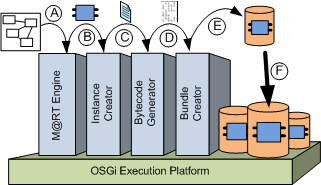
\includegraphics[width=.6\textwidth]{part2/pics/toolchain3.png}
  \caption{Instance creation tool chain}
  \label{fig:instanceToolChain}
%  \vspace{-5mm}
\end{figure}

The creation of an instance is realized as presented on figure~\ref{fig:instanceToolChain}. From the model (step A), a new instance is queried by the Model@Runtime engine(step B) to an instance creator. This instance creator can be a Java code generator, an XML generator, or whatever. The instance creator then asks for the bytecode generator to compile the instance. This compilation can be realized with ASM\footnote{http://asm.ow2.org} for Java code, handled by Spring for an XML file, etc. Step D consists in packaging the bytecode in a bundle. Step E makes it available for the runtime platform. The last step installs the instance bundle in the system.\\

Mapped on OSGi bundles, component instances can offer services to other components in the component model, or to other bundles on the OSGi platform. This facility makes it possible to dynamically expose instances on application-level protocols. This role is supported by the {\it Wrappers} layer described in section~\ref{sec:wrappers}.

\vspace{1cm}
\section{Wrappers}
\label{sec:wrappers}
\begin{wrapfigure}{r}{60mm}
  \vspace{-5mm}
  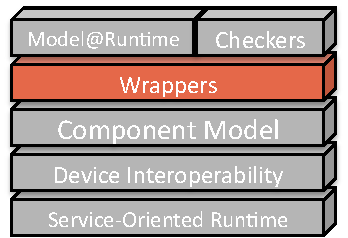
\includegraphics[width=60mm]{part2/pics/layers/Wrappers.pdf}
%  \caption{!!!!!! NO CAPTION !!!!!!}
  %\label{fig:agePyramidEU272009}
  \vspace{-5mm}
\end{wrapfigure}


The wrappers layer takes advantage of the component model layer, which makes it possible to dynamically and automatically wrap devices into several current and future application level protocols. For instance, \gls{upnp}, \gls{dpws} or \gls{dlna} are such kinds of protocols. Their implementations is often too heavy to be implanted into the devices themselves. The role of this layer is thus to export all devices for free, on several protocols. Rather than offering an automatic publication mechanism to a selected protocol, the wrappers layer offers a means to publish any component to any protocol. Each component can thus be accessible using as many protocols as there are wrappers. This approach has been presented in~\cite{Nain08a}.\\

{\bf Component Model {\it versus} Third party}\\
Wrappers need to obtain information about the devices present in a given deployment. This information can be retrieved in two ways.\\
(1) The wrapper is designed as a component. As a consequence, it can monitor the current model of the running system by asking the {\it Model@Runtime} layer. Any change in the model implies that the wrapper check new devices and removed ones. Another benefit of this approach is that a wrapper is considered as a classical component. The model can thus manage it as any other component.\\
(2) The wrapper is built as a third party application, running on the same platform. In this case, the wrapper monitors registrations of services in the OSGi context. Each time a device registers a service, this service is made accessible through the protocol handled by the wrapper. This approach has two drawbacks. Firstly, the export and use of services are not visible in the model. A device can thus be removed while in use through an application protocol. Secondly, the life cycles of the services exported on the application protocol depend on the registration and unregistration of the device's services. Since no dependency is expressed in the model, the life-cycle management of exported services has to be handled 'by hand' by the wrapper.\\

{\bf Reversed drivers}\\
A wrapper is created for each application level protocol. Just as for devices' drivers, the deployment of a wrapper is required for each application protocol to be addressed. Each wrapper monitors the current application to detect addition or removal of devices. For each device, the wrapper takes on the role of a proxy and handles communications to and from the application level protocol.


\section{Summary}
The model used by the Model@Runtime engine has been augmented with the introduction of the component model described in section~\ref{sec:componentModel}.\\
The service-oriented architecture of the runtime makes it possible to cope with evolutions and adaptations, since bundles can be installed and updated with no need to restart the system. These facilities are exploited by the Model@Runtime layer, which comes with tools and methods to address the evolutions, variability, adaptations and safety of the application. However, these properties could not have been used without the creation of a new component model inspired by electronic components. This component model improves flexibility and enables the connection of heterogeneous components, while keeping a high level of reliability thanks to checkers. The Device Interoperability and Wrappers layers provide abstractions of manufacturers' specificities and free publications on application level protocols respectively, to promote interoperability and openness.



\chapter{Outcomes}
\label{ch:outcomes}

This chapter aims at providing a bit more details about the outcomes of this thesis in terms of implementation and tools. The first section gives quite general information about the implementation of this component model and provides some metrics. The second and last section of this chapter classifies the component model according to the classification proposed by Crnkovic in~\cite{Crnkovic_1374:2007}.

\section{Implementation}

The ideas presented in this thesis have been tested and improved in several situations and contexts thanks to an implementation.\\

{\bf EnTiMid} has grouped together all separated layers to provide a first running implementation of the component model and tools. Because of the context, EnTiMid targets the creation and realization of software applications in the domain of Home Automation. However, ideas presented in this thesis are more general and applicable in other domains such as Machine-To-Machine or automotive industry.\\
The arrival of a new PhD student in the team incited to rethought and rebuild the software solution.\\

{\bf Kevoree} has inspired and integrated ideas developed in this thesis and in EnTiMid, to create a more general purpose software development environment. This generalization enables the use of these ideas in several projects and implementation in the team. It also allows for future specializations or extensions of this work. As for EnTiMid, it has been re-factored to specialize Kevoree for a use in the domain of HomeAutomation.\\

EnTiMid concentrates in integrating new ideas like Models@Runtime and the flexible component model. Thus, an iterative process on top of an OSGi platform led to the creation of a new component model with its implementation. However, this implementation allowed us to change, drop, refactor our code to validate our ideas, which could have been more difficult by extending existing platforms.\\
If the implementation is home-made, the structure of components in our component model is close to existing models, making it possible to develop extensions to integrate the contributions of this thesis to existing models.\\


\section{Impact on the development process}

The use of \enti{} impacts the development process at several levels. To describe this impact, this section details the elements manipulated and the tools available for different development phases.

\begin{figure}[h!]
  \centering
  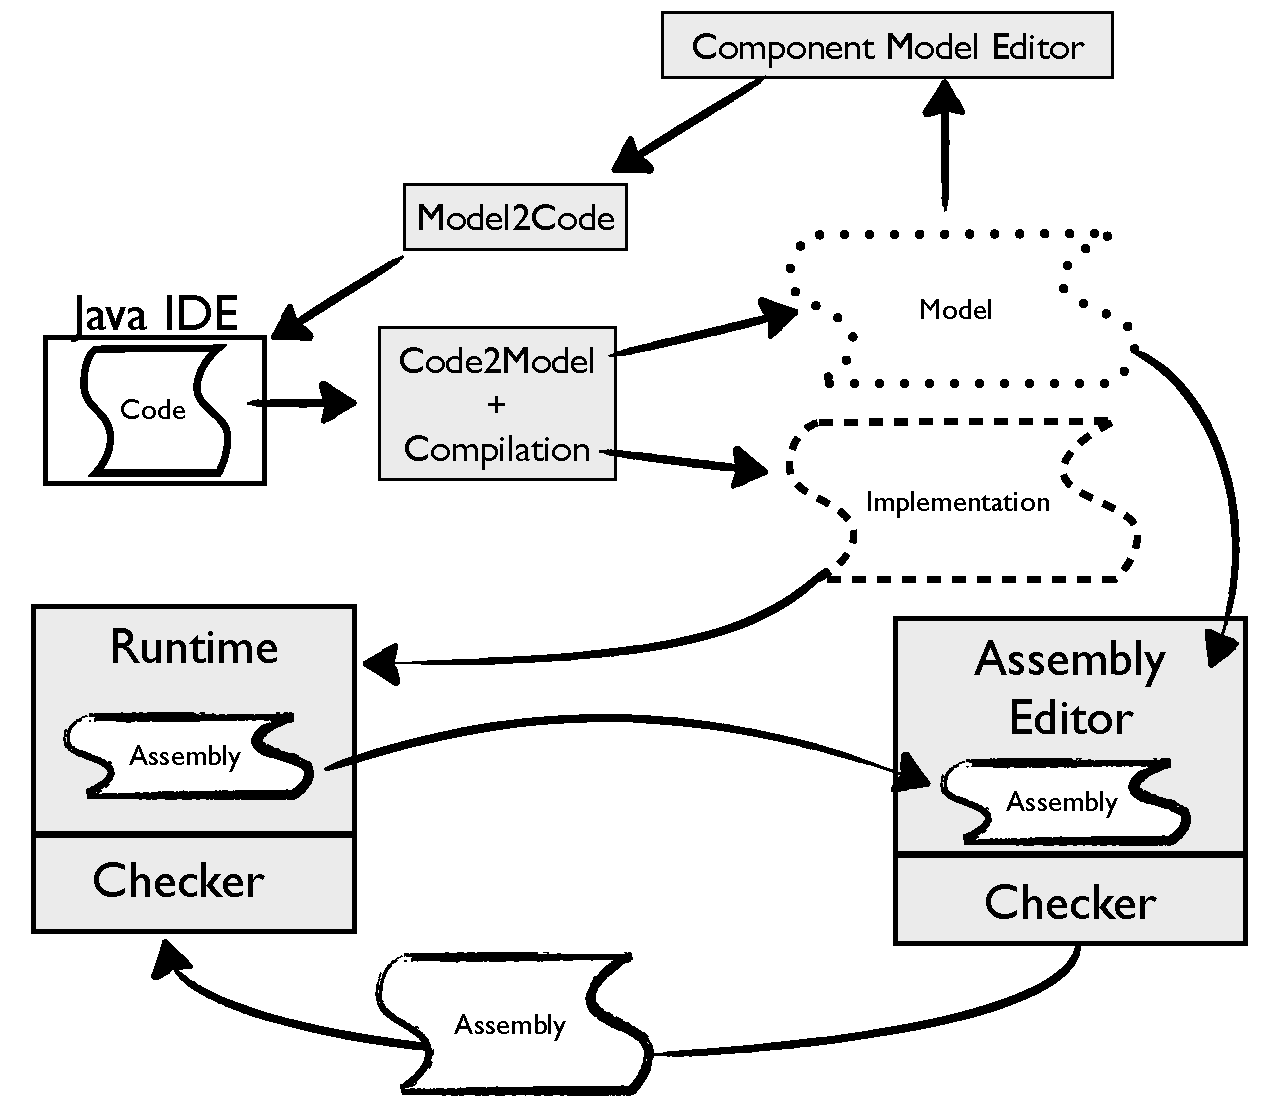
\includegraphics[width=.8\textwidth]{part2/pics/Chain.pdf}
  \caption{EnTiMid development chain}
  \label{fig:devchain}
\end{figure}


\subsection{Component development}

Since the component model is highly permissive, component developers cannot make any assumption on the context of use of the component. Components are thus required to be well protected against wrong usages, bad or missing parameters.\\
The use of annotations to describe the model and map ports and methods, makes easier the migrations of code, refactorings and evolutions of implementations.
The model of a component described by the annotations can be different from its actual implementation, because several ports can be mapped on a single method.
Moreover, if a component offers a service port (implementing a specific interface), the component's implementation class does not have to (but still can) implement the interface of the provided service. The only required thing is to map all methods of the service interface to operation in the code.\\
These mappings provide flexibility to component models and their implementations.\\

The compilation chain, represented on figure~\ref{fig:devchain} by the "Code2Model" box, automatically checks for mandatory life-cycle methods and verifies that all methods of all ports are actually mapped on implementation methods. In the same time, the chain extracts the models of the components by parsing the annotations. These models are then embedded in the archive containing the sources compiled in the same compilation process. This guaranties the model-code consistency by construction.\\

As presented on top of figure~\ref{fig:devchain}, a component editor can be used to create or modify an existing component model. This model of component is then synchronized with the code thanks to a tool, "Model2Code engine", which generates a component's implementation skeleton or updates the annotations in an existing code.

\subsection{Application design}

In a design process, the component model of EnTiMid and the assembly tools make it possible to connect heterogeneous components, such as actual devices, functions, or services available through internet. Since the model is very flexible and permissive, designer can try and deploy any combination of components, unless checkers in the assembly tool or in the runtime reject the model. The bottom of figure~\ref{fig:devchain} illustrates this.\\

According to the domain of application, checkers can be specialized to avoid assemblies identified as leading to failures. Moreover, checkers can be adapted to the current user of the application and give more authorizations to an engineer, and more restrictions to the end-user for instance.\\

Finally, runtime checkers have to be specialized to reject models requiring resources not available on the platform (serial port connections for instance).\\

In case an adaptation or an evolution is required, the model of the running system is always available and can be collected directly from the runtime. Once updated, the model of the system can be sent to the runtime for a adaptation of the actually running application.


\section{Metrics}
The table~\ref{table:metrics} provides some lines of code metrics of Kevoree and EnTiMid. These metrics have been measured on Kevoree 1.5.0-SNAPSHOT and EnTiMid 3.0.0-SNAPSHOT on the 23rd November 2011. The counting was realized using Cloc\footnote{http://cloc.sourceforge.net/} by considering only files contained in the {\it src} folder of each project. Thus generated code has not been counted. A Maven\footnote{http://maven.apache.org/} plugin recursively launched the counting on sub-modules of a top-project, and aggregated the results.\\

\begin{table}[h!]
\centering
\begin{tabular}{l||>{\centering}m{1cm}|>{\centering}m{1.5cm}|>{\centering}m{1.5cm}|>{\centering}m{1.5cm}|>{\centering\arraybackslash}m{1.5cm}}
Project & Scala & Java & Total & Part & Value \\
\hline \hline
Kevoree-Core & 8143 & 344 & 8487 & 11,54\% & 979,3 \\
Kevoree-Tools & 8483 & 6255 & 14738 & 22,22\% & 3274,65 \\
Kevoree-Extra(ecore) & 1275 & 126 & 1401 & 50\% & 700,5 \\
\hline \hline
EnTiMid-Core & 0 & 445 & 445 & 85\% & 378,25 \\
EnTiMid-Tools & 82 & 315 & 3197 & 75\% & 2397,75 \\
EnTiMid-Library & 0 & 2065 & 2065 & 80\% & 1652 \\
EnTiMid-Extra & 0 & 1091 & 1091 & 85\% & 927,35 \\
\end{tabular}\\
\caption{Lines of code metrics of Kevoree and EnTiMid}
\label{table:metrics}
\end{table}
\vspace{-0.2cm}

Kevoree and EnTiMid have been implemented in mixed Java and Scala languages. The table provides an indication of my participation in the different projects of the implementation. The complement has been realized in collaboration with other PhD students of the team.\\
The core of Kevoree embeds the implementation of the meta-model, a loader, a serializer, a cloner and some utility classes grouped in a framework used for both runtime management and design of components.\\
Kevoree-Tools contains a graphical editor for components and assemblies, model and code synchronization tools and the definition of a scripting language to ease the management of models.\\
Since, Kevoree can be seen as a generalization of EnTiMid, the most important part of development in EnTiMid was paid in creating component libraries and extra APIs wrapping, specialized for home automation technologies and devices. For demonstration purposes, several additional tools had also been realized.

\section{Classification}

Crnkovic proposed in~\cite{Crnkovic_1374:2007} a classification framework "to increase the understanding of concepts and easier differentiate component models". This section aims at classifying the component model of this thesis according to this classification. Four dimensions are considered in~\cite{Crnkovic_1374:2007}. Each dimension is presented in a separated subsection.\\
The tables presented here have been extracted (for existing component models) from the Crnkovic classification, and completed to integrate EnTiMid. The component models selected for this extraction are also present in the state-of-the-art section.

\subsection{Lifecycle}
~\vspace{-0,5cm}
\begin{table}[h!]
\centering
{\scriptsize 
\begin{tabular}{|>{\centering}m{.12\textwidth}||>{\centering}m{.20\textwidth}|>{\centering}m{.20\textwidth}|>{\centering}m{.16\textwidth}|>{\centering\arraybackslash}m{.16\textwidth}|}
\hline
Component Models & Modeling & Implementation & Packaging & Deployment \\
\hline
EJB & N/A & Java & EJB-Jar files & At run-time \\
\hline
Fractal & ADL-Like Language(Fractal ADL, Fractal IDL)\\ Annotations(Fractlet) & Java(in Julia, Aokell)\\ C/C++(in Think)\\ .Net lang(in FracNet) & File system based Repository & At run-time \\
\hline
OSGi & N/A & Java & Jar-files (bundles) & At run-time and at compilation \\
\hline\hline
EnTiMid & Graphical and Textual ADL, Annotations(CDL) & Java, Scala & Jar-files(bundles) Repositories & At run-time and at compilation \\
\hline
\end{tabular}
}
\caption{The Lifecycle dimension}
\label{tabl:classifLifeycle}
\end{table}
\vspace{-0,2cm}

EnTiMid proposes several tools for editing components and applications. Developments can be done in Java and/or Scala, and deployments (based on OSGi mechanisms) are realized using Jar files and repositories. This deployment can be done while the system is running.

\subsection{Constructs}
~
\vspace{-0,5cm}
\begin{table}[h!]
\centering
{\scriptsize 
\begin{tabular}{|>{\centering}m{.12\textwidth}|| >{\centering}m{.16\textwidth}| >{\centering}m{.17\textwidth}| >{\centering}m{.12\textwidth}| >{\centering}m{.14\textwidth}| >{\centering\arraybackslash}m{.11\textwidth}|}
\hline
Component Models & Interface type & Provides/Require distinction & Distinctive Features & Interface Language & Interface Levels \\
\hline
EJB & Operation-based & No & N/A & Java Programming Language + Annotations & Syntactic \\
\hline
Fractal & Operation-based & Yes & Component Interface, Control Interface & IDL, Fractal ADL, Java, C, Behavioral Protocol & Syntactic, Behavior \\
\hline
OSGi & Operation-based & Yes & Dynamic Interfaces & Java & Syntactic \\
\hline\hline
EnTiMid & Port-based & Yes & Types Specified in Interfaces & Java, Annotation, other & Syntactic, Semantic \\
\hline
\end{tabular}
}
\caption{The Constructs dimension - Interface Specifications}
\label{table:classifConstIface}
\end{table}

Each port in EnTiMid can be specified independently, making interfaces types port-based. The model also differentiates between provided and required ports. The types of ports are specified in the component model and their parameters also, which is a particularity. The language to describe the interface can be Java(for services ports) or just annotations (for message ports). In case of message ports, they handle the semantic of the call; otherwise it is a syntactic interface level.

\begin{table}[h!]
\centering
{\scriptsize
\begin{tabular}{|>{\centering}m{.12\textwidth}||>{\centering}m{.28\textwidth}|>{\centering}m{.23\textwidth}|>{\centering}m{.10\textwidth}|>{\centering\arraybackslash}m{.12\textwidth}|}
\hline
\multirow{2}{.13\textwidth}{\centering Component Models} & \multirow{2}{*}{Interaction Styles} & \multirow{2}{*}{Communication Type} & \multicolumn{2}{c|}{Binding Type} \\
\cline{4-5}
& & & Exogenous & Hierarchical \\
\hline
EJB & Request Response & Synchronous, Asynchronous & No & No \\
\hline
Fractal & Multiple Interaction Styles & Synchronous, Asynchronous & Yes & Delegation, Aggregation \\
\hline
OSGi & Request Response, Triggering & Synchronous & No & No \\
\hline\hline
EnTiMid & Multiple Interaction Styles & Synchronous, Asynchronous & Yes & Delegation \\
\hline
\end{tabular}
}
\caption{The Constructs dimension - Interaction}
\label{table:classifConstInteract}
\vspace{-0,2cm}
\end{table}


Interaction style between components depends on the channel used. The channel supports the interaction and can act as a blocking service call, as a trigger or even with some callback mechanisms. Thus communications can be synchronous or asynchronous according to the channel chosen. Bindings are made explicit by the concept of channels. In case of a composition, the behavior of the binding is dependent of the implementation of the composite component. As of today, the unique composition mechanism available in EnTiMid is the inheritance, and can be considered as a delegation in this case.

\subsection{Extra-Functional Properties}

\begin{table}[h!]
\centering
{\scriptsize
\begin{tabular}{|>{\centering}m{.12\textwidth}||>{\centering}m{.30\textwidth}|>{\centering}m{.28\textwidth}|>{\centering\arraybackslash}m{.13\textwidth}|}
\hline
Component Models & Management of EFP & Properties Specification & Composition and Analysis support \\
\hline
EJB & Exogenous System wide(D) & N/A & N/A \\
\hline
Fractal & Exogenous per collaboration(C) & Ability to add properties (by adding "property" controllers) & N/A \\
\hline
OSGi & Endogenous per collaboration(A) & N/A & N/A \\
\hline\hline
EnTiMid & Exogenous System wide(D) & Metrics<key,value> values updated at run-time & Handled by pluggable reasoners \\
\hline
\end{tabular}
}
\caption{The Extra-Functional Properties dimension}
\label{table:classifProp}
\end{table}

Working with a model at run-time makes it possible to dynamically get the value of a metric on a running component. Metrics are specified on and updated by components in the model. Theses metrics are <key,value> pairs and can represent any interesting data on the component behavior. Their analysis can be performed locally or remotely by reasoner capable of making a decision from a given model extracted from the running system.

\subsection{Domains}

\begin{table}[h!]
\centering
{\scriptsize
\begin{tabular}{|>{\centering}m{.13\textwidth}||c|c|c|}
\hline
Component Models & General Purpose & Specialized & Generative \\
\hline
EJB & X & & \\
\hline
Fractal & X & & X \\
\hline
OSGi & X & & \\
\hline\hline
EnTiMid & & X & X \\
\hline
\end{tabular}
}
\caption{The Domains dimension}
\label{table:classifDomains}
\end{table}

Dedicated to the domain of Home Automation and \gls{aal}, EnTiMid is clearly specialized. Kevoree, on its side, can be considered as more generic.
